\documentclass[11pt,a4paper,oneside]{book}
\usepackage[usenames,dvipsnames,svgnames,table]{xcolor}
\usepackage[a4paper, portrait, margin=1.1in]{geometry}
\usepackage{url}
\usepackage{makeidx}
\usepackage{listings}
\usepackage{graphicx}
\usepackage{fancyhdr}
\usepackage{fancyvrb}
\usepackage{parskip}
\usepackage{chngpage}
\usepackage{lmodern}
\usepackage{caption}
\usepackage{subcaption}
\usepackage{afterpage}
\usepackage{pdflscape}
\usepackage{capt-of}
\usepackage[utf8]{inputenc}
\usepackage[toc,page,header]{appendix}
% \usepackage[usenames,dvipsnames]{color}

\usepackage[none]{hyphenat} % FIXME REMOVE FOR FINAL DOCUMENT	

\newcommand{\HRule}{\rule{\linewidth}{0.5mm}}
\renewcommand{\familydefault}{\sfdefault}

\renewcommand{\arraystretch}{1.5} % Stretch spacing between table rows


\definecolor{lightgray}{rgb}{.95,.95,.95}
\definecolor{darkgray}{rgb}{.4,.4,.4}
\definecolor{green}{rgb}{.2,.6,.0}
\definecolor{lightblue}{rgb}{.0,.5,.7}
\definecolor{purple}{rgb}{0.6, .1, 0.62}

\lstdefinelanguage{JavaScript}{
  keywords={typeof, new, true, false, catch, function, return, null, catch, switch, var, if, in, while, do, else, case, break, throw},
  keywordstyle=\color{blue}\bfseries,
  ndkeywords={exports, this},
  ndkeywordstyle=\color{lightblue}\bfseries,
  identifierstyle=\color{black},
  sensitive=false,
  comment=[l]{//},
  morecomment=[s]{/*}{*/},
  commentstyle=\color{green}\ttfamily,
  stringstyle=\color{purple}\ttfamily,
  morestring=[b]',
  morestring=[b]"
}

\lstdefinelanguage{KRE}{
  keywords={select, when, setting, with, http},
  keywordstyle=\color{blue}\bfseries,
  ndkeywords={rule},
  ndkeywordstyle=\color{lightblue}\bfseries,
  identifierstyle=\color{black},
  sensitive=false,
  morecomment=[s]{re\#}{\#},
  commentstyle=\color{green}\ttfamily,
  stringstyle=\color{purple}\ttfamily,
  morestring=[b]',
  morestring=[b]"
}

% \lstdefinelanguage{JSON}{
%   identifierstyle=\color{black},
%   sensitive=false,
%   stringstyle=\color{purple}\ttfamily,
%   morestring=[b]',
%   morestring=[b]"
% }

% \definecolor{numb}{RGB}{150, 150, 150}
% \definecolor{delim}{RGB}{20,105,176}

% \lstdefinelanguage{JSON}{
%   identifierstyle=\color{black},
%   sensitive=false,
%   stringstyle=\color{purple}\ttfamily,
%   morestring=[b]',
%   morestring=[b]",
%     literate=
%      *{0}{{{\color{numb}0}}}{1}
%       {1}{{{\color{numb}1}}}{1}
%       {2}{{{\color{numb}2}}}{1}
%       {3}{{{\color{numb}3}}}{1}
%       {4}{{{\color{numb}4}}}{1}
%       {5}{{{\color{numb}5}}}{1}
%       {6}{{{\color{numb}6}}}{1}
%       {7}{{{\color{numb}7}}}{1}
%       {8}{{{\color{numb}8}}}{1}
%       {9}{{{\color{numb}9}}}{1}
%       % {\{}{{{\color{delim}{\{}}}}{1}
%       % {\}}{{{\color{delim}{\}}}}}{1}
%       % {[}{{{\color{delim}{[}}}}{1}
%       % {]}{{{\color{delim}{]}}}}{1}
% }

\lstdefinelanguage{RDF}{
  keywords={on, insert, if, do, delete, let, in},
  keywordstyle=\color{blue}\bfseries,
  % keywords=[2]{delta},
  % keywordstyle=[2]\color{green}\bfseries,
  ndkeywords={document, resource},
  ndkeywordstyle=\color{lightblue}\bfseries,
  identifierstyle=\color{black},
  sensitive=false,
  comment=[l]{//},
  morecomment=[s]{/*}{*/},
  commentstyle=\color{green}\ttfamily,
  stringstyle=\color{purple}\ttfamily,
  morestring=[b]',
  morestring=[b]"
}

\lstdefinelanguage{N3}{
  alsoletter=?,
  keywords={ ?x },
  keywordstyle=\color{blue}\bfseries,
  ndkeywords={exports, this},
  ndkeywordstyle=\color{lightblue}\bfseries,
  identifierstyle=\color{black},
  sensitive=false,
  comment=[l]{//},
  morecomment=[s]{/*}{*/},
  commentstyle=\color{green}\ttfamily,
  stringstyle=\color{purple}\ttfamily,
  morestring=[b]',
  morestring=[b]"
}

\lstdefinelanguage{XChange}{
  keywords={TRANSACTION, on, end, in, insert, from},
  keywordstyle=\color{blue}\bfseries,
  ndkeywords={xchange, var, resource},
  ndkeywordstyle=\color{lightblue}\bfseries,
  identifierstyle=\color{black},
  sensitive=false,
  comment=[l]{//},
  morecomment=[s]{/*}{*/},
  commentstyle=\color{green}\ttfamily,
  stringstyle=\color{purple}\ttfamily,
  morestring=[b]',
  morestring=[b]"
}

\lstset{
  language=JavaScript,
  % backgroundcolor=\color{lightgray},
  extendedchars=true,
  basicstyle=\footnotesize\ttfamily,
  showstringspaces=false,
  showspaces=false,
  numbers=left,
  numberstyle=\tiny,
  numbersep=9pt,
  tabsize=2,
  breaklines=true,
  showtabs=false,
  captionpos=b,
  aboveskip=10pt,
  belowskip=10pt,
  xleftmargin=.3in,
  % frameround=tttt,
  boxpos=t
}


\makeatletter
\def\PY@reset{\let\PY@it=\relax \let\PY@bf=\relax%
    \let\PY@ul=\relax \let\PY@tc=\relax%
    \let\PY@bc=\relax \let\PY@ff=\relax}
\def\PY@tok#1{\csname PY@tok@#1\endcsname}
\def\PY@toks#1+{\ifx\relax#1\empty\else%
    \PY@tok{#1}\expandafter\PY@toks\fi}
\def\PY@do#1{\PY@bc{\PY@tc{\PY@ul{%
    \PY@it{\PY@bf{\PY@ff{#1}}}}}}}
\def\PY#1#2{\PY@reset\PY@toks#1+\relax+\PY@do{#2}}

\expandafter\def\csname PY@tok@gd\endcsname{\def\PY@tc##1{\textcolor[rgb]{0.63,0.00,0.00}{##1}}}
\expandafter\def\csname PY@tok@gu\endcsname{\let\PY@bf=\textbf\def\PY@tc##1{\textcolor[rgb]{0.50,0.00,0.50}{##1}}}
\expandafter\def\csname PY@tok@gt\endcsname{\def\PY@tc##1{\textcolor[rgb]{0.00,0.27,0.87}{##1}}}
\expandafter\def\csname PY@tok@gs\endcsname{\let\PY@bf=\textbf}
\expandafter\def\csname PY@tok@gr\endcsname{\def\PY@tc##1{\textcolor[rgb]{1.00,0.00,0.00}{##1}}}
\expandafter\def\csname PY@tok@cm\endcsname{\let\PY@it=\textit\def\PY@tc##1{\textcolor[rgb]{0.25,0.50,0.50}{##1}}}
\expandafter\def\csname PY@tok@vg\endcsname{\def\PY@tc##1{\textcolor[rgb]{0.10,0.09,0.49}{##1}}}
\expandafter\def\csname PY@tok@m\endcsname{\def\PY@tc##1{\textcolor[rgb]{0.40,0.40,0.40}{##1}}}
\expandafter\def\csname PY@tok@mh\endcsname{\def\PY@tc##1{\textcolor[rgb]{0.40,0.40,0.40}{##1}}}
\expandafter\def\csname PY@tok@go\endcsname{\def\PY@tc##1{\textcolor[rgb]{0.53,0.53,0.53}{##1}}}
\expandafter\def\csname PY@tok@ge\endcsname{\let\PY@it=\textit}
\expandafter\def\csname PY@tok@vc\endcsname{\def\PY@tc##1{\textcolor[rgb]{0.10,0.09,0.49}{##1}}}
\expandafter\def\csname PY@tok@il\endcsname{\def\PY@tc##1{\textcolor[rgb]{0.40,0.40,0.40}{##1}}}
\expandafter\def\csname PY@tok@cs\endcsname{\let\PY@it=\textit\def\PY@tc##1{\textcolor[rgb]{0.25,0.50,0.50}{##1}}}
\expandafter\def\csname PY@tok@cp\endcsname{\def\PY@tc##1{\textcolor[rgb]{0.74,0.48,0.00}{##1}}}
\expandafter\def\csname PY@tok@gi\endcsname{\def\PY@tc##1{\textcolor[rgb]{0.00,0.63,0.00}{##1}}}
\expandafter\def\csname PY@tok@gh\endcsname{\let\PY@bf=\textbf\def\PY@tc##1{\textcolor[rgb]{0.00,0.00,0.50}{##1}}}
\expandafter\def\csname PY@tok@ni\endcsname{\let\PY@bf=\textbf\def\PY@tc##1{\textcolor[rgb]{0.60,0.60,0.60}{##1}}}
\expandafter\def\csname PY@tok@nl\endcsname{\def\PY@tc##1{\textcolor[rgb]{0.63,0.63,0.00}{##1}}}
\expandafter\def\csname PY@tok@nn\endcsname{\let\PY@bf=\textbf\def\PY@tc##1{\textcolor[rgb]{0.00,0.00,1.00}{##1}}}
\expandafter\def\csname PY@tok@no\endcsname{\def\PY@tc##1{\textcolor[rgb]{0.53,0.00,0.00}{##1}}}
\expandafter\def\csname PY@tok@na\endcsname{\def\PY@tc##1{\textcolor[rgb]{0.49,0.56,0.16}{##1}}}
\expandafter\def\csname PY@tok@nb\endcsname{\def\PY@tc##1{\textcolor[rgb]{0.00,0.50,0.00}{##1}}}
\expandafter\def\csname PY@tok@nc\endcsname{\let\PY@bf=\textbf\def\PY@tc##1{\textcolor[rgb]{0.00,0.00,1.00}{##1}}}
\expandafter\def\csname PY@tok@nd\endcsname{\def\PY@tc##1{\textcolor[rgb]{0.67,0.13,1.00}{##1}}}
\expandafter\def\csname PY@tok@ne\endcsname{\let\PY@bf=\textbf\def\PY@tc##1{\textcolor[rgb]{0.82,0.25,0.23}{##1}}}
\expandafter\def\csname PY@tok@nf\endcsname{\def\PY@tc##1{\textcolor[rgb]{0.00,0.00,1.00}{##1}}}
\expandafter\def\csname PY@tok@si\endcsname{\let\PY@bf=\textbf\def\PY@tc##1{\textcolor[rgb]{0.73,0.40,0.53}{##1}}}
\expandafter\def\csname PY@tok@s2\endcsname{\def\PY@tc##1{\textcolor[rgb]{0.73,0.13,0.13}{##1}}}
\expandafter\def\csname PY@tok@vi\endcsname{\def\PY@tc##1{\textcolor[rgb]{0.10,0.09,0.49}{##1}}}
\expandafter\def\csname PY@tok@nt\endcsname{\let\PY@bf=\textbf\def\PY@tc##1{\textcolor[rgb]{0.00,0.50,0.00}{##1}}}
\expandafter\def\csname PY@tok@nv\endcsname{\def\PY@tc##1{\textcolor[rgb]{0.10,0.09,0.49}{##1}}}
\expandafter\def\csname PY@tok@s1\endcsname{\def\PY@tc##1{\textcolor[rgb]{0.73,0.13,0.13}{##1}}}
\expandafter\def\csname PY@tok@sh\endcsname{\def\PY@tc##1{\textcolor[rgb]{0.73,0.13,0.13}{##1}}}
\expandafter\def\csname PY@tok@sc\endcsname{\def\PY@tc##1{\textcolor[rgb]{0.73,0.13,0.13}{##1}}}
\expandafter\def\csname PY@tok@sx\endcsname{\def\PY@tc##1{\textcolor[rgb]{0.00,0.50,0.00}{##1}}}
\expandafter\def\csname PY@tok@bp\endcsname{\def\PY@tc##1{\textcolor[rgb]{0.00,0.50,0.00}{##1}}}
\expandafter\def\csname PY@tok@c1\endcsname{\let\PY@it=\textit\def\PY@tc##1{\textcolor[rgb]{0.25,0.50,0.50}{##1}}}
\expandafter\def\csname PY@tok@kc\endcsname{\let\PY@bf=\textbf\def\PY@tc##1{\textcolor[rgb]{0.00,0.50,0.00}{##1}}}
\expandafter\def\csname PY@tok@c\endcsname{\let\PY@it=\textit\def\PY@tc##1{\textcolor[rgb]{0.25,0.50,0.50}{##1}}}
\expandafter\def\csname PY@tok@mf\endcsname{\def\PY@tc##1{\textcolor[rgb]{0.40,0.40,0.40}{##1}}}
%\expandafter\def\csname PY@tok@err\endcsname{\def\PY@bc##1{\setlength{\fboxsep}{0pt}\fcolorbox[rgb]{1.00,0.00,0.00}{1,1,1}{\strut ##1}}}
\expandafter\def\csname PY@tok@kd\endcsname{\let\PY@bf=\textbf\def\PY@tc##1{\textcolor[rgb]{0.00,0.50,0.00}{##1}}}
\expandafter\def\csname PY@tok@ss\endcsname{\def\PY@tc##1{\textcolor[rgb]{0.10,0.09,0.49}{##1}}}
\expandafter\def\csname PY@tok@sr\endcsname{\def\PY@tc##1{\textcolor[rgb]{0.73,0.40,0.53}{##1}}}
\expandafter\def\csname PY@tok@mo\endcsname{\def\PY@tc##1{\textcolor[rgb]{0.40,0.40,0.40}{##1}}}
\expandafter\def\csname PY@tok@kn\endcsname{\let\PY@bf=\textbf\def\PY@tc##1{\textcolor[rgb]{0.00,0.50,0.00}{##1}}}
\expandafter\def\csname PY@tok@mi\endcsname{\def\PY@tc##1{\textcolor[rgb]{0.40,0.40,0.40}{##1}}}
\expandafter\def\csname PY@tok@gp\endcsname{\let\PY@bf=\textbf\def\PY@tc##1{\textcolor[rgb]{0.00,0.00,0.50}{##1}}}
\expandafter\def\csname PY@tok@o\endcsname{\def\PY@tc##1{\textcolor[rgb]{0.40,0.40,0.40}{##1}}}
\expandafter\def\csname PY@tok@kr\endcsname{\let\PY@bf=\textbf\def\PY@tc##1{\textcolor[rgb]{0.00,0.50,0.00}{##1}}}
\expandafter\def\csname PY@tok@s\endcsname{\def\PY@tc##1{\textcolor[rgb]{0.73,0.13,0.13}{##1}}}
\expandafter\def\csname PY@tok@kp\endcsname{\def\PY@tc##1{\textcolor[rgb]{0.00,0.50,0.00}{##1}}}
\expandafter\def\csname PY@tok@w\endcsname{\def\PY@tc##1{\textcolor[rgb]{0.73,0.73,0.73}{##1}}}
\expandafter\def\csname PY@tok@kt\endcsname{\def\PY@tc##1{\textcolor[rgb]{0.69,0.00,0.25}{##1}}}
\expandafter\def\csname PY@tok@ow\endcsname{\let\PY@bf=\textbf\def\PY@tc##1{\textcolor[rgb]{0.67,0.13,1.00}{##1}}}
\expandafter\def\csname PY@tok@sb\endcsname{\def\PY@tc##1{\textcolor[rgb]{0.73,0.13,0.13}{##1}}}
\expandafter\def\csname PY@tok@k\endcsname{\let\PY@bf=\textbf\def\PY@tc##1{\textcolor[rgb]{0.00,0.50,0.00}{##1}}}
\expandafter\def\csname PY@tok@se\endcsname{\let\PY@bf=\textbf\def\PY@tc##1{\textcolor[rgb]{0.73,0.40,0.13}{##1}}}
\expandafter\def\csname PY@tok@sd\endcsname{\let\PY@it=\textit\def\PY@tc##1{\textcolor[rgb]{0.73,0.13,0.13}{##1}}}
%\expandafter\def\csname PY@tok@err\endcsname{}

\def\PYZbs{\char`\\}
\def\PYZus{\char`\_}
\def\PYZob{\char`\{}
\def\PYZcb{\char`\}}
\def\PYZca{\char`\^}
\def\PYZam{\char`\&}
\def\PYZlt{\char`\<}
\def\PYZgt{\char`\>}
\def\PYZsh{\char`\#}
\def\PYZpc{\char`\%}
\def\PYZdl{\char`\$}
\def\PYZhy{\char`\-}
\def\PYZsq{\char`\'}
\def\PYZdq{\char`\"}
\def\PYZti{\char`\~}
% for compatibility with earlier versions
\def\PYZat{@}
\def\PYZlb{[}
\def\PYZrb{]}
\makeatother

% How deep numbering is applied to titles
% \setcounter{secnumdepth}{3}
\setcounter{tocdepth}{1}

% Prepare the word index
\makeindex

% Prepare header and footer
\pagestyle{fancy}
\fancyhf{}
\rhead{\footnotesize\leftmark}
\lfoot{Towards Reactive Information Systems and their Services}
\rfoot{\thepage}
\renewcommand{\headrulewidth}{0.3pt}
\renewcommand{\footrulewidth}{0.3pt}

% Apply page style also to chapter's first page
\makeatletter
\renewcommand\chapter{\if@openright\cleardoublepage\else\clearpage\fi
  \thispagestyle{fancy}%
  \global\@topnum\z@
  \@afterindentfalse
  \secdef\@chapter\@schapter}
\makeatother

\setlength{\parindent}{15pt}
% \setlength{\parskip}{.5\baselineskip}%

\begin{document}

\frontmatter
	\begin{titlepage}
\begin{center}

% \title{\huge \textbf{Towards The Reactive Web}\vspace*{15 mm}}
% %\subtitle{Master Thesis Report}
% \date{\today}
% %\date{}
% %\author{Dominic Bosch \\ Departement Mathematics and Computer Science \\ University of Basel}
% \author{\fontsize{11}{9}\selectfont
% Master Thesis\\
% \vspace*{10 mm}\\
% Dominic Bosch\\
% Departement Mathematics and Computer Science\\
% University of Basel
% }
% \maketitle

\vspace*{4cm}
\HRule \\[0.4cm]
{ \huge \bfseries Towards Reactive Information Systems \\ and their Services \\[0.4cm] }
% { \huge \bfseries Towards The Reactive Web \\[0.4cm] }
\HRule \\[1.5cm]

% \textsc{\Large Departement Mathematics and Computer Science}\\[0.5cm]

\vspace*{.5cm}
\textit{\textsc{\LARGE Master Thesis}}\\
\vspace*{2.5cm}

% Author and supervisor
\begin{minipage}{0.4\textwidth}
\begin{flushleft} \large
\emph{Author:}\\
Dominic \textsc{Bosch}
\end{flushleft}
\end{minipage}
\begin{minipage}{0.4\textwidth}
\begin{flushright} \large
\emph{Supervisors:} \\
Prof. Dr.~Helmar \textsc{Burkhart}\\
Dr.~Martin \textsc{Guggisberg}
\end{flushright}
\end{minipage}

\vfill

% Bottom of the page
{\large May 15, 2014} \\[1.5cm]



% \textsc{\LARGE University of Basel}\\

\includegraphics[width=0.15\textwidth]{figures/unilogoschwarz}~\\[1cm]
\end{center}
\end{titlepage}

	\chapter*{Abstract}
The \textrm{\gls{web}} is a rapidly growing information universe, consisting of \textrm{\glspl{infosystem}} that provide access to heterogeneous services.
A large part of those \textrm{\glspl{infosystem}} are dynamic.
Changes in their \textrm{\gls{infospace}} trigger events, which can be detected.
Moreover, such changes can also be imposed onto the \textrm{\gls{infospace}} over the appropriate services.
If appropriate services exist to access such an \textrm{\gls{infosystem}} for read and write operations, we are able to orchestrate it.
By adopting the \textrm{\acrlong{eca} (\acrshort{eca})} paradigm to \textrm{\glspl{infosystem}}, we are able to introduce an event-based conceptual model.
This model allows the detection of events and the dispatching of actions according to predefined rules, thus imposing reactivity on top of or between \textrm{\glspl{infosystem}}.
Current approaches that use the \textrm{\acrshort{eca}} paradigm focus on action imposition on local storage, while we aim to impose actions on the hetereogeneous services of existing \textrm{\glspl{infosystem}}.
This model is not limited to the \textrm{\gls{web}}, but can include any accessible \textrm{\glspl{infosystem}}.

In our work we introduce a prototype system, which uses the \textrm{\gls{web}}'s programmability to impose reactivity on top of it.
We also underline the importance of the, currently little, support of \textrm{\glspl{webservice}} for event callback addresses, the so called \textrm{\glspl{webhook}}.
They are the only way for real-time event delivery to remote systems and free them from expensive polling for changes.
Through our prototype it is possible to orchestrate \textrm{\glspl{webservice}} based on an \textrm{\acrlong{eda} (\acrshort{eda})}, a method which pushes towards the vision of real-time reactive \textrm{\glspl{infosystem}}.
We list some example use cases for our conceptual model, as well as use cases that have been implemented in our prototype system.

\vspace{2cm}
All research results\footnote{https://github.com/dominicbosch/msc-liveweb} and the prototype system project\footnote{https://github.com/dominicbosch/webapi-eca} are stored on two public accessible \textrm{GitHub} repositories.
	\chapter*{Acknowledgment}
I would like to express my deep gratitude to my master thesis advisor, Prof. Dr. Helmar Burkhart, for his patience and constant encouragement to keep going further.
I also want to thank Dr. Martin Guggisberg for his very helpful advices and hints to existing technologies.
Besides my advisors, I would like to thank the members of the research group: Danilo Guerrera,
Antonio Maffia, Alexander Gr\"oflin and Robert Frank for their help, many interesting discussions and inputs.

I would like to thank my parents Silvia and Peter Bosch for their love, patience and financial support on my journey.
Special thanks go to my sister Svenja, her husband Andreas and their seven months old son Nico, who all kept me going with their joyfulness and irresistble smiling.
Finally I would like to thank my partner Kathrina Hagnauer for her patience and endless love.
	\tableofcontents

\mainmatter
	
\chapter{Introduction}

\textit{\textbf{TODO: use the word task or workflow?}}

The Web is an ever growing institution, in all aspects that it covers.
Research on behalf of the Web attracts a great deal of attention, even more since modern life is already impossible without it.

\textit{Just imagine how you will get food without money because the credit card reader can't establish a connection to the bank.
If you still got some cash you'll have to save it, since banks will not work anymore when the Web is gone. \textbf{(Really necessary?)}}

The number of information and functionality providers for the Web is growing in the whole spectrum from bigger computing centers down to smaller devices.
Computing centers, growing in size and quantity, allow for massive amounts of data to be stored and accessed, but they also enable the construction and accessibility of more complex functionalities.
Ever smaller devices provide informations and functionalities to the Web, through their quickly increasing number.
Many of them are even providing access to the Web itself and thus leverage the effect of the growing Web.
For example mobile phones can act as a hotspot to grant Web access to others through \textrm{WiFi}.
\index{Web of Things}
All the smart \textrm{Things} with access to the Web start to form the \textrm{Web of Things}.
This can be every\textrm{Thing} from a temperature sensor to all electronical devices within a house.
These \textrm{Things} do not only provide sensor data but they can also be easily controlled through the Web.

Confronted with this rapid growth of the Web, an increasing number of human beings is exposed to it in their daily life and they get literally flooded with data and possibilities to govern them.
Even though they have access to all these services and data in the Web, they often lack the knowledge, necessary time or right approach to weave them together.
Users need ways to get appropriate informations, in the right moment, automatically and in a condensed matter that suits them best.
They have to be able to automate tedious tasks, e.g. detecting relevant changes in information resources and react on behalf of such changes.
\textit{\small{More concrete example?}}
This requires the identification of and filtering for user-specific information, appropriate timing, assembly and preprocessing of different information resources and finally the forwarding of outcomes to services in the web. 

Users don't want to be bound to specific services or applications, they want to use their preferred one, which they are used to and which helps them best to fulfill their needs.
Some of these services in the web offer ways to spread their data to other pre-defined services, but in very limited amount and parametrization.
Therefore users end up mashing informations or functionalities from different locations within the Web by hand.
This often means to execute similar tasks repeatedly by hand.
Moreover the completion of such a task suffers from latency due to the deferred detection of the initialization or because the user is just not able to execute the work at that time.
And also if the bits and pieces that form such a task could be separated, it is likely that some parts could be reused for other tasks or even by other people to get similar work done.

Since the data and the functionality already exists in the Web, the users could automate their work to some extent by orchestrating services and data.
Even though the access to services and data gets simpler, the average user is not able to fully exploit the Web.
Another challenge is that often a lot of effort needs to be invested, in understanding how the service works, before it can be fully exploited.
It is desirable to retain manageable mashing of servcies and data, while still exploiting their full potential.
There are many attempts that go towards an easy to orchestrate the Web, but they are either complicated to weild themselves or mere data copy or mashup approaches.

A big part of the informations, that become available to the users, are short-lived informations corresponding to certain state changes, and can therefore be modeled as events.
In this thesis we to introduce an event-driven conceptual model that enables the programmability of the Web and thus imposes reactivity on the Web.
We claim the whole Web as our information space, in which we listen for triggered events and in which we execute actions as a result.
Such an user-specific reactivity allows a personalization of the whole Web and a tool to govern its information flood.
This would allow users to orchestrate the Web in an intuitive way and to tailor reactivity to their needs.
Current orchestration approaches concentrate on data flow rather than on event flow, which are mere data copy/paste tasks than reactivity.
This makes us believe that an event-based conceptual model can overcome certain shortcomings of the existing solutions.

\begin{figure}[!ht]
  \centering
  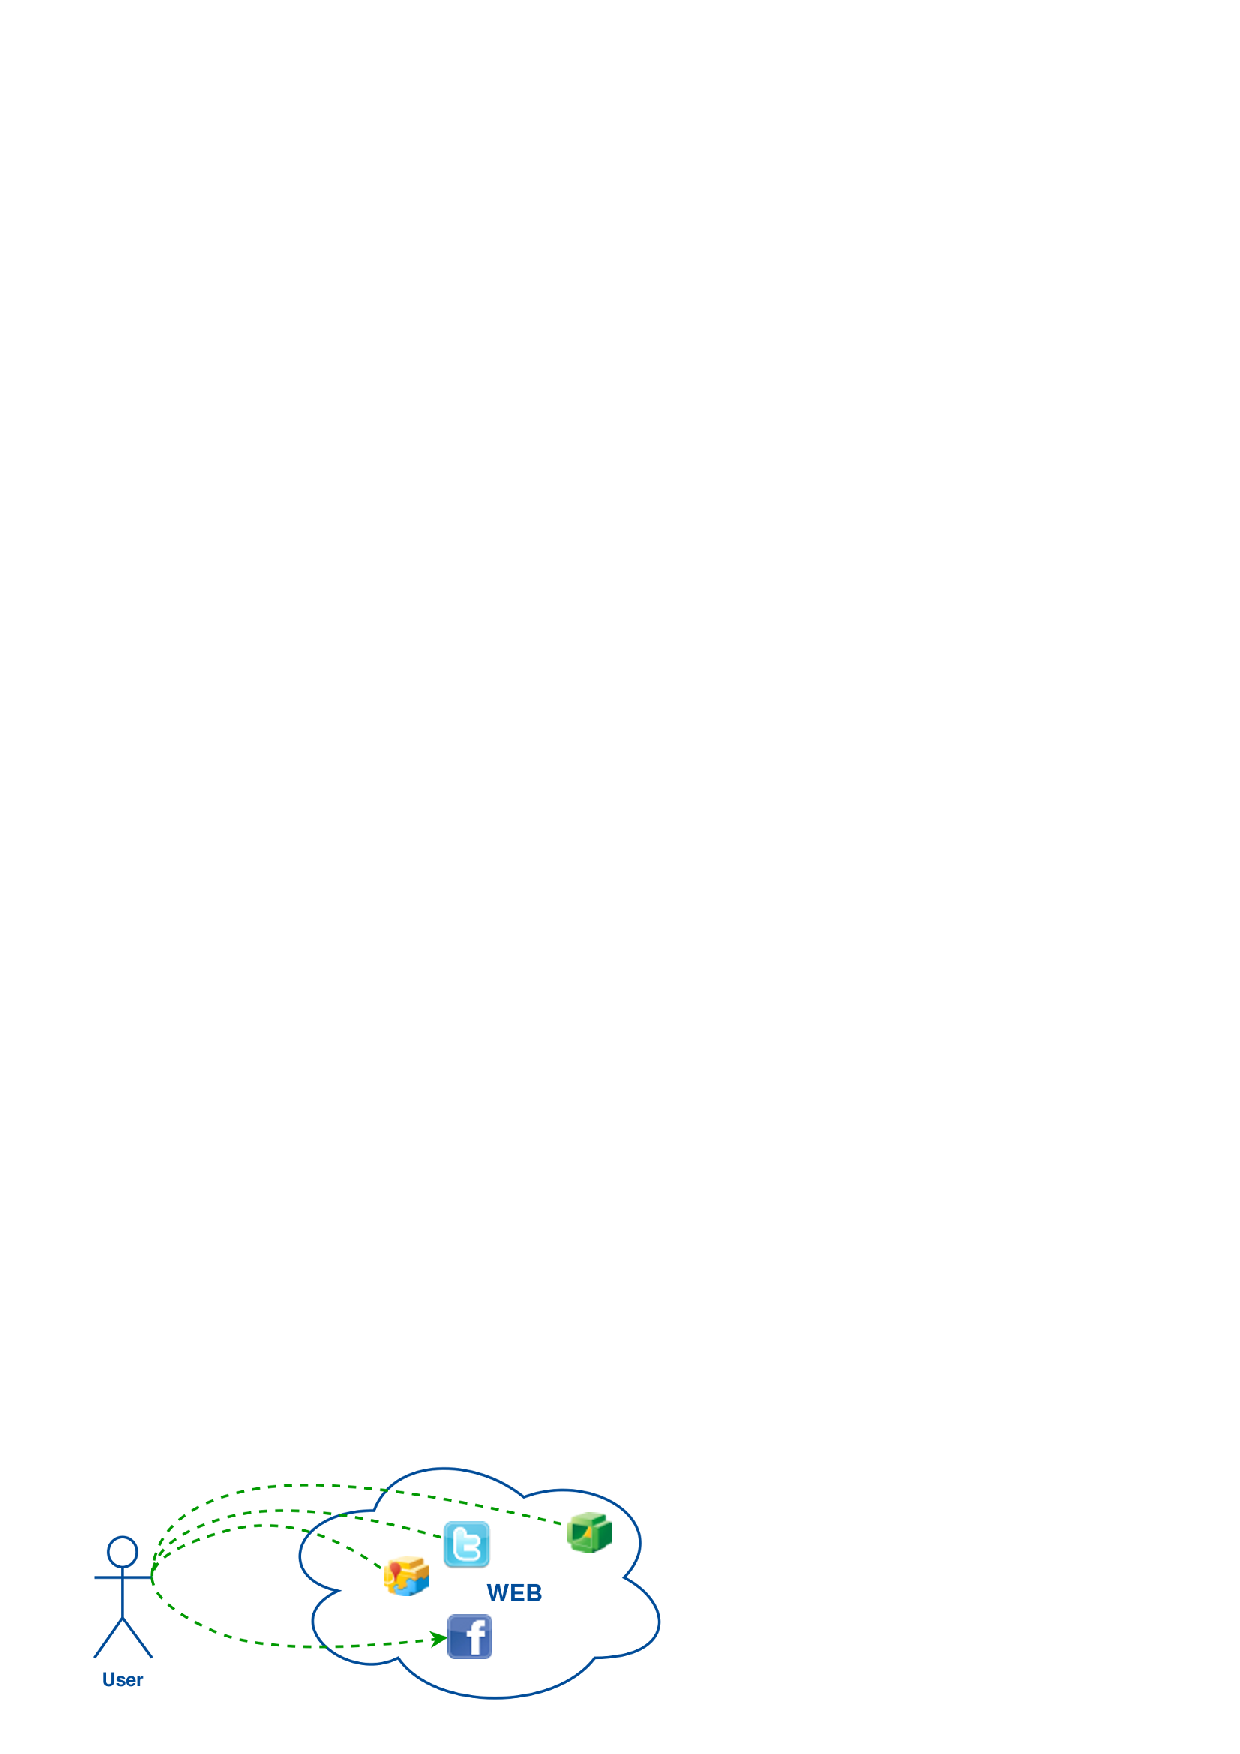
\includegraphics[width=0.7\textwidth]{figures/UsersWeildServicesInTheWeb}
  \caption{Users mashup the Web's Information and Data}
  \label{fig:UsersWeildServicesInTheWeb}
\end{figure}
\textit{\small{ewwww ugly figure....\\
TODO show more concrete example with aha effect, light bulb. maybe parallel or serial events that turn into a result}}


	\chapter{Related Work}

\index{Web Service}
\index{Web API}
% Web Services – Opportunities and Challenges
% NICOLETA DAVID, CLAUDIA-GEORGETA CARSTEA,
% IOAN-GHEORGHE RATIU, LUCIAN PATRASCU, DANIELA DAMIAN
%Web Services term refers to available programmatic interfaces that are used in the World Wide Web for application-to-application communication.

% An approach to develop a layered architecture from software engineering, principles was proposed by Gerber et al. [23], referred to as the Comprehensive, Functional, Layered (CFL) architecture for the Semantic Web. C
 % - Gerber A., van der Merwe A. and Barnard A. Towards a Semantic Web Layered Architecture. In Proceedings of IASTED International Conference on Software Engineering, (SE2007), Innsbruck, Austria. IASTED 2007. ISBN 978-0-88986-641-6, pp. 353–362.

% http://benchmarksgame.alioth.debian.org/u64/benchmark.php?test=all&lang=java&lang2=v8&data=u64 seem to back our findings
% https://www.paypal-engineering.com/2013/11/22/node-js-at-paypal/ as well
% https://vividcortex.com/blog/2013/12/09/analysis-of-paypals-node-vs-java-benchmarks/ interpretes above results:
% My guess is that Node is encouraging good programmer practices in terms of scalability, and Java less so. In other words, programmers probably have to work less hard to avoid bad scalability bottlenecks in Node than in Java.


% XML SOAP WSDL UDDI RDF OWL
% microformats: xhtml rss

% http://www.w3.org/TR/ws-gloss/: A Web service is a software system designed to support interoperable machine-to-machine interaction over a network.
% http://www.informationweek.com/from-edi-to-xml-and-uddi-a-brief-history-of-web-services/d/d-id/1012008?
% -> Common Object Request Broker Architecture, Distributed Component Object Model, Unix Remote Procedure Call, and Java Remote Method Invocation. Each of those technologies failed to gain significant market share or enough momentum to succeed.
% CORBA , RMI
% XML officially became a standard in February 1998, when the World Wide Web Consortium announced that XML 1.0 had reached draft recommendation status: suitable for deployment in applications.
% SOAP won over WDDX (Web Distributed Data Exchange)
% SOAP 1.0, its specification for a standardized message-passing protocol based on XML.
% REST
% TODO dienste services WebAPI belegen mit referenzen wo begriff wie gebraucht wird
% Begriffe festnageln, definieren
Data and functionalities in the web were always accessible via web services, whatever this means.
reengineering of services in the beginning
with standardised REST API's we got to Web API, easy access and understandable


The fast evolving web has brought up a trend towards easy to master interfaces to services, the so called Web APIs.
They do not only provide access to mere services but whole applications that allow access over Web APIs.
These trending Web APIs benefit from a RESTful architecture which predominantly uses HTTP and thus relies on the most basic and powerful operations and the basis of the Web itself, the HTTP protocol. 

% TODO Enough on Web API's?

% quick (handling/mastering) accessible services and even whole web applications through so called Web APIs.
% Web APIs provide powerful tools to govern data and functionality in the web independently of any user interface from the service provider.
% The relatively
% Allowing access to these services via API is increasingly popular and allows to mash up these services

% Practically all services flood the user with events
% The web should be event driven, that's why we need an engine that deals with events and makes the web reactive
% There's still the challenge of filtering
% What's important to whom
% Plus the user needs to have tools to combine and add programmability to the combination,( such as conditions, selection of provided arguments and so on)

% % TODO Event Trigger
% \index{Event}
% \index{Event Trigger}

% % TODO Actions
% \index{Actions}

% % TODO engine
% \index{Engine}


% % TODO Webhooks
% \index{Webhooks}

% TODO Categorize Related Work!

\index{Mashups}
Mashups combine information and functionality of more than one web service in a single place.
The mashing up of such web services allows data to be enhanced with new informations, processing / refinement of the information, or even ways to interact with them, e.g. through Google Maps.
Simple functions from different sources can be combined into more powerful ones, which influence data and services in a way their founders eventually didn't even think of.
Web service mashups have been developped ever since services in the web started to exist and were accessible in a more or less convenient way.
We introduce Paul Rademacher as an example for how recent the invention of web service mashups are.
He's one of the first inventors of such a web service mashup.
In the same year after Google Maps came up in 2005, he invented a site\cite{wwwRademacherOne,wwwRademacherTwo} that displayed Craigslist houses on a Google Map.
With no Google Maps API at that time, he needed time and skills to reverse engineer Google Map's functionalities.


A large number of such "static" mashups were and are still developped.
They are static in the way that they aggregate a fixed (and mostly low) number, of either data or functionality resources, to provide an enhanced resource in a specialized domain.
Of course Mashups can be mashed up again, to provide even more sophisticated functionality and data.
Some latest example Mashups, taken from the ProgrammableWeb\cite{wwwProgrammableWeb} directory, are:

\begin{itemize}
  \item Wifi and Plugs\cite{wwwWifiAndPlugs}: MapBox, Google Docs and Import.io API's used to display where Wi-Fi and plugs are available in London.
  \item MapLight\cite{wwwMapLight}: GovTrack.us and OpenSecrets API's used to combine political results with financial contributions to show how capital contributions affect voting.
  \item Shared Count\cite{wwwSharedCount}: Facebook, LinkedIn, Pinterest and Twitter API's used to display informations about how well spread a URL is on social media sites.
\end{itemize}

In the past few years, research and development for platforms to allow users to flexibly mashup Web APIs got attention.
% Web API mashups
With IFTTT and Zapier, two platforms have evolved out of this process.
Users that register on those platforms are provided with a multitude of Web API functions that act as event triggers and such that are used to execute actions.
The user is then free to combine these event triggers and actions in the way it suits best, creating helpful Web API mashups on their own.

% Since this is a quite new field the why and how is hidden from the research.
% you need events
% you need rules / rule language

% TODO REST paper, Craigslist artcile / Paper



\index{Rule}
\index{Engine}
\index{Rule Language}

It turns out that Web API mashing up is not able to bring reactivity to the web.
They are merely aggregations of services that only provide data or functions but no write possibilities such as web applications provide.
% only limited functionalty
% limited parametrization
% often only read / new aggregation / no writes
% TODO find mashup that does writes in a system! (not existing right?)

Thus 

% TODO
% To allow user-defined Web API mashups, a rule language is required which is capable to express ECA Rules. 


% TODO
% ECA
% \index{ECA}

%TODO Table with categorization of Rule languages

Several different rule languages have been developped for different purposes over the last years and they vary grately in their purpose.
% terms of usability for ECA Rules together with Web API mashups.
A compilation of research on different emerging rule-based languages and technologies \cite{2009-Paschke_Boley-RCER.pdf} gives an oveview over such efforts.
We examined different existing rule languages with respect to a certain use case to identify its applicability for reactivity in the web. % TODO find other word as applicability
The use case is defined such that the rule needs to suffice the ECA paradigm:

\begin{itemize}
  \item Event: Receipt of an Email
  \item Condition: Check for a certain sender
  \item Action: Store it remotely via a Web API
\end{itemize}

We defined an email event which the rule languages need to be able to process.
The JSON representation of the given email event as depicted in the appendix. %is shown in Listing~\ref{lstemail}.

% FIXME Leave out what was not inspiring!

\index{RDF}
\index{XML}
An early ECA Rule Language for XML repositories\cite{Papamarkos03event-condition-actionrule} was postulated in 2003 and was picked up by many researches afterwards. It was designed to react on insert and delete events within XML repositories and as an action change XML documents.


Now apart from implementing a rules engine, we would also need to add an XML document event manager which interpretes and pushes events into the XML file \emph{inbound\_queue.xml}. Then again this instance would interprete the ouptuts of the ECA engine, which would theoretically manifest in other XML documents, and produce meaningful actions on remote hosts. This wouldn't be an architecture which has its focus on the solution of our use case and, as a result, add complexity and create an unnecessary overhead.

\index{Notation 3}
To make the lengthy RDF definitions smaller and more readable, Notation 3\cite{wwwn3} was designed and announced in 2005. Through the implies operator(=\textgreater) an "event" can be connected to an "action", both expressed in RDF's subject, predicate, object notation, which makes the expression of ECA rules a complicated and not very intuitive task. A solution to our use case would look as follows:

This language is used to express relations between entities and thus not really suitable for our use case, since we would require another interpreter to infer the actions. But concepts and ideas of the work that was done in these consortias could eventually still find influence into our solution.

\index{XChange}\index{Xcerpt}
The rule language XChange\cite{2005-Patranjan-TLE.pdf} was the outcome of the REWERSE (\cite{wwwRewerse}, Reasoning on the Web with Rules and Semantics) project, which was funded by the EU and Switzerland. Their work influenced a number of future research. The language was designed to add reactive behaviour to a "static" web which is represented through XML resources. Thus we have action logics to alter such resources through insertions and deletions. Since we aim to utilize web API's for our rule language we need a more generic approach which adds flexibility in term of the API provided. But the thorough research done with the language XChange holds valuable concepts, especially in terms of temporal evet composition. This could be a rule according to our use case:


But XChange is designed to access other resources in an action and thus provides powerful tools:

\index{JSON Rules}
In 2008 \emph{JSON Rules}~\cite{2008-Giurca_Pascalau-JSON_Rules.pdf} was introduced as a language to easily react on specific DOM tree compositions.
The usage of JavaScript allowed them to provide simple functions which could be called directly by the actions, thus abstracting functionality from the language.
This key concept found influence into our language as it allows different layers of abstractions.
Through this it is possible to provide generic functions for expert user as well as very limited functions with only few possibilities for parameterization to be used by unexperienced persons.
A drawback of this language is its binding to DOM tree events, where we would want to react on any events happening in the world.
Also the temporal composition to complex events is not a subject of their work and needs further attention.


\index{KRL}
A most recent (2011) open-source development is the Kinetic Rules Engine together with the Kinetics Rule Language~\cite{bookTheLiveWeb}.
It is built for the purpose of adding reactivity to the cloud.
The language is based on declarative syntax, enriched with imparative elements.
But it is a tedious task to get into a whole new language and their caveats.
\emph{authorization?}


\index{RuleML}
The basis of \emph{RuleML}~\cite{2006-Boley-RuleML.pdf} is datalog, a language in the intersection of SQL and Prolog.
In 2012 the \emph{Reaction RuleML}~\cite{2012-Paschke_etal-ReactionRuleML.pdf} language incorporated several different types of rules into the RuleML syntax, to establish a uniform syntax and interchangability of rules.
\emph{Reaction RuleML} is a valuable resource in terms of manifold research that has been done in the domain of rule languages, but the syntax is not user-friendly.


R2ML allows usage for RuleML together with many other dialects. Really!?

% TODO RULE ENGINES!

%\section{Conclusion}
Most of the examined rule languages are designed for the interchangability of rules between different service providers. We do not attempt to jump into this domain but we rather pick up important concepts to manifest web API's as first class citizens of our rule language. This allows the ad-hoc design and implementation of reactive rules between existing web API's without the need for their cooperation in setting up their endpoint in a special way.

% TODO Rechtfertigung wieso nicht verwendet
% Java EE und KRL nicht anwendbar


% TODO performance artikel / paper ueber node.js
	
% Rahmenbedingungen
% Vorzuege
% Notwendigkeiten
% Architektur
% Schema: Zeit / Verteiltheit
% Steckbrief von Prototyp erstellen
 % was muss man ausfüllen um UC zu erstellen?
% why are we now suddenly responsive? we loosened up certain things
% point out where events happen, triggered and received



\chapter{Conceptual Model for Reactive Information Systems and their Services}
The challenges and opportunities arising with the growth of the Web in terms of volume and complexity inspired our research towards the reactive Web.
Therefore our starting point were the studies of related work in the context of reactivity on the Web, event composition and programmability of the Web.
In the last chapter, we pointed out how they received a lot of attention and provide powerful tools to orchestrate the rapidly growing Web.
By combining existing research in these fields we developped a conceptual model, which allows to impose smart reactivity to any \textrm{\gls{infospace}}.
Even though our initial set of \textrm{\glspl{infospace}} was thought to consist of \textrm{\glspl{webresource}}, our model is applicable to any \textrm{\gls{infosystem}} whose \textrm{\gls{infospace}} can be accessed and altered over interfaces, i.e. services.
Thus we introduce our conceptual model for reactive \textrm{\glspl{infosystem}} and their services in this chapter.

\begin{figure}[!ht]
  \centering
  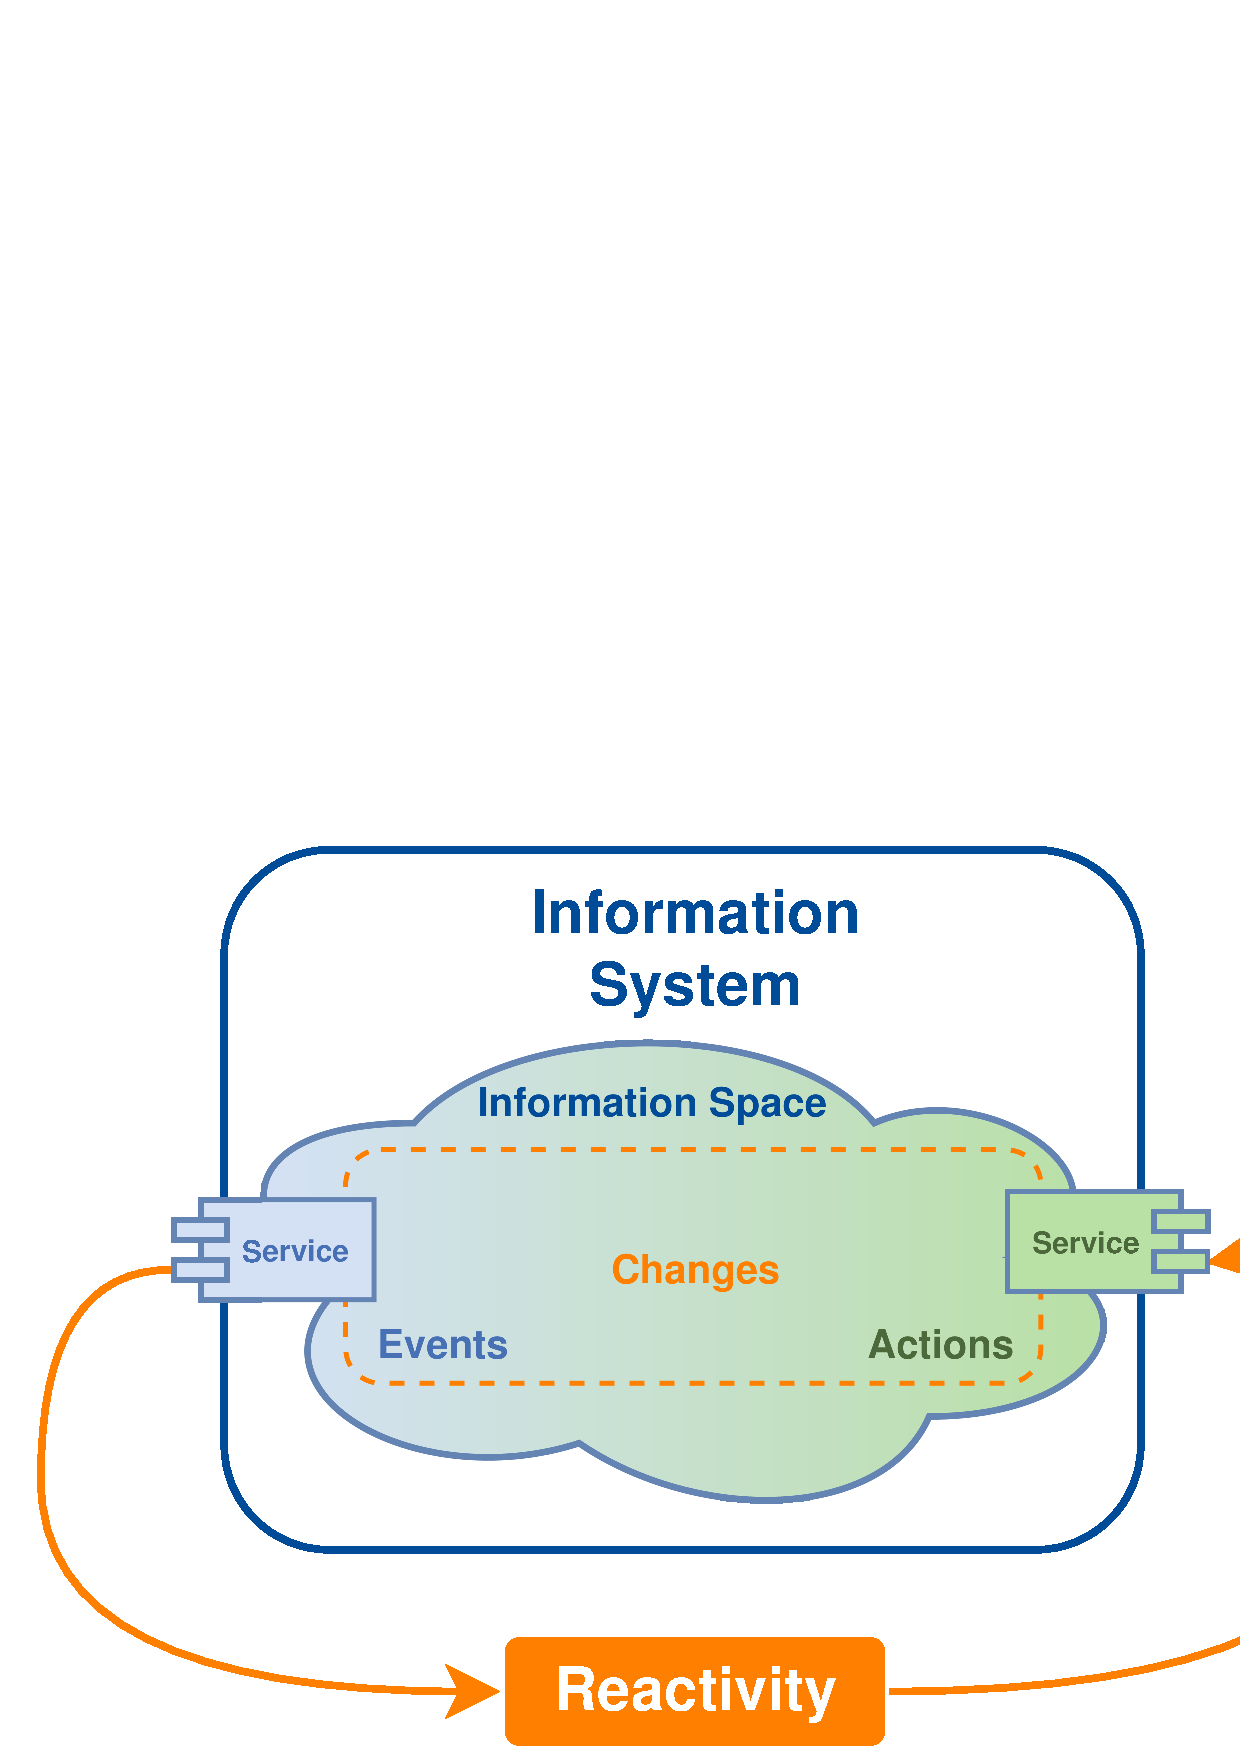
\includegraphics[width=0.8\textwidth]{figures/IS_InformationSpace}
  \caption{Reactivity imposed on Information Systems and their Information Space over Services}
  \label{fig:IS_InformationSpace}
\end{figure}
Data changes within an \textrm{\gls{infosystem}} can be detected and imposed from the outside, if proper interfaces exist, the services.
We model the detection of data changes as events, and the inflicting of such changes as actions, as shown in Figure \ref{fig:IS_InformationSpace}.
Through this we are able to introduce an event-based model that is capable to detect events and react on behalf of them by imposing actions on the same or another \textrm{\gls{infospace}}.
A more precise distinction of the important modules for such a reactivity imposing entity is displayed in Figure \ref{fig:Standard-Model-Template}, and we will introduce each module in this chapter.
\begin{figure}[!ht]
  \centering
  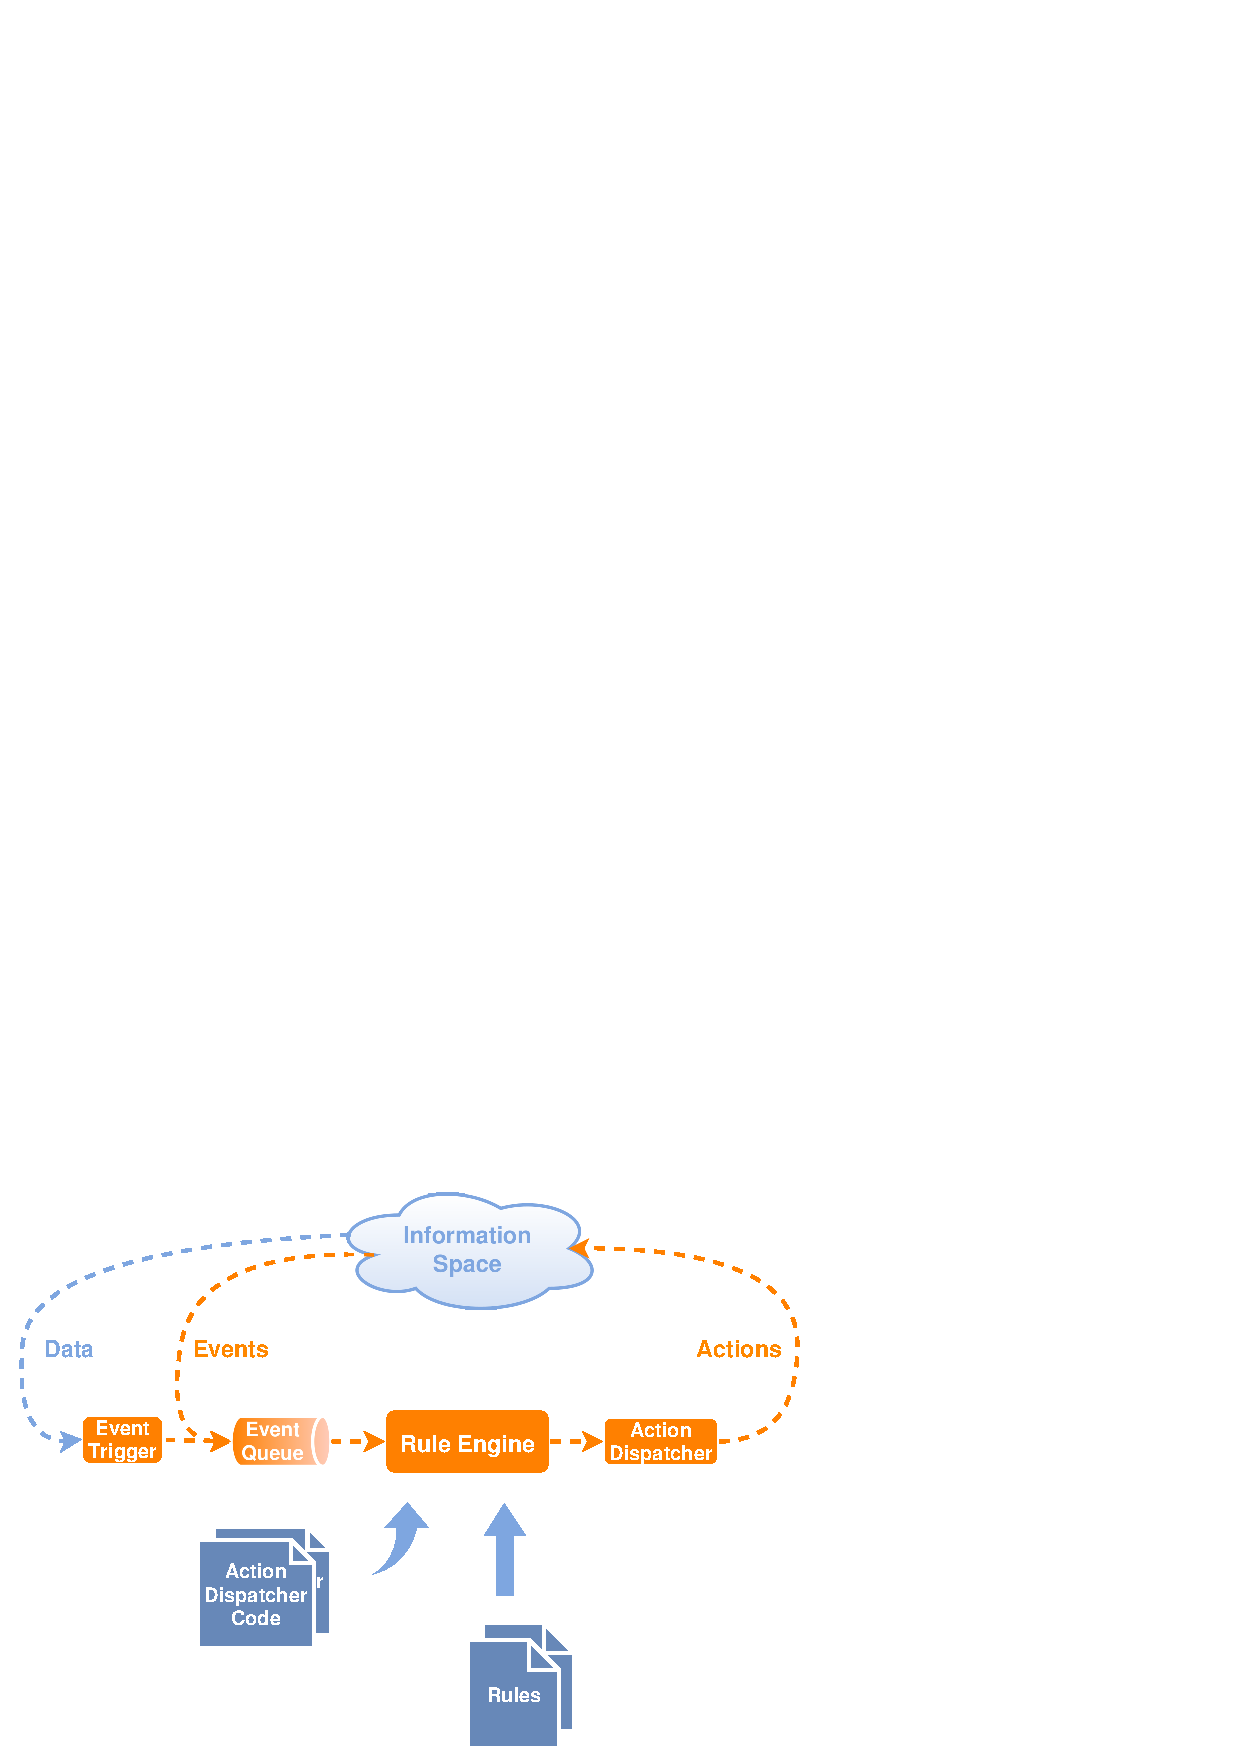
\includegraphics[width=0.7\textwidth]{figures/Standard-Model-Template}
  \caption{Conceptual Model for Reactive Information Systems and their Services}
  \label{fig:Standard-Model-Template}
\end{figure}



\section{From Physical Events to Virtual Events}
We introduced the \textrm{\gls{webofthings}} in the last chapter, where smart devices gain access to the Web.
It is based on the \textrm{Internet of Things} which mostly dealt with the incorporation of sensor networks into the Internet on the network level.
Such sensors bring the physical world directly into the virtual world.
This transfer pictures an important difference between physical and virtual events.
In physics, and in particular relativity, an event indicates a physical situation or occurrence, located at a specific point in space and time.
While physical events correspond to a physical situation which is located at a specific point in space and time, virtual events primarily consist of implicit parameters, i.e. a name and occurrence time.
These virtual events can be anywhere within \textrm{\glspl{infosystem}} at any point in time and thus their actual location differs most certainly from its occurrence location.
But virtual events also have explicit parameters which correspond to all available information about the event.
As soon as events are transfered into the virtual world the afore mentioned location information turns into explicit parameters.
Therefore wherever a virtual event is, it has a name, an occurence time and most likely some explicit parameters attached to it.
If the virtual event is of a physical nature, it has a physical location, if it is of a virtual nature it is likely associated with a virtual origin.
Since in our model events are changes in data, they can be virtually anything, e.g. measurements, changes on a static webpage, changes of the object behind a \textrm{\gls{webservice}} or also a login attempt.
% TODO TABELLE Ort/Kultur(fussball/Apple, weltweit)/Saisonal(kalender)/Internet (ortlos, github)
% ceremony
% competition
% meeting
% disaster
% event horizon
% extinction event
% festival
% grouped events
% happening
% impact evetn
% media event
% mental event
% news
% party
% phenomenon
% sporting event
% synchronization


\section{Capturing Events from Information Systems}
The optimal case for an event-driven system which requires events from an \textrm{\gls{infosystem}} is, that events are triggered within the \textrm{\glspl{infosystem}} and then immediately communicated to interested external systems such as our envisioned reactivity imposing system.
But our research has shown that such \textrm{\glspl{infosystem}} are often passive and rarely provide ways for external systems to announce interest in changes of their data.
For example in the context of \textrm{\glspl{webresource}}, many of them provide service access to data but do not actively communicate changes to interested parties.
This is where the upcoming concept of \textrm{\glspl{webhook}} comes into play.
Only through them we are able to provide nearly real-time reactivity without risking huge costs of continuously polling for changes over all \textrm{\glspl{infospace}}.
We envision a future where the whole Web is event driven and events are directed to any system, which is interested in them.
This would be the optimal case for effective real-time notifications and thus reactivity on the Web.
But still we need to incorporate polling for changes into our model, in order to cope for the widely spread passiveness of \textrm{\glspl{infosystem}} which is likely to never thoroughly vanish.
Wherever an \textrm{\gls{infosystem}} is not capable to provide events over services, we can use all the accessible data and detect changes in it, and as a result model them as events in order to feed them into our model.
In our model the polling for changes is incorporated in the \textrm{Event Trigger} modules.
Those are flexible modules that have the proper tools to access any \textrm{\gls{infosystem}} service and therefore its \textrm{\gls{infospace}} and are capable of identifying changes in the data.
For example the \textrm{\gls{www}}, as envisioned by Tim Berners-Lee\cite{DBLP:journals/en/Berners-LeeCGP92}, is an information universe of interlinked documents, that a user can browse through.
Through our model, we can pull changes in the data on the \textrm{\gls{www}}, i.e. document changes, and turn them into events.
These events which are derived from changes in the data of \textrm{\gls{infosystem}} are then fed into the \textrm{Event Listener}.
The \textrm{Event Listener} also receives events directly from he \textrm{\glspl{infosystem}} which are capable to communicate events to external systems.
It queues all events and forwards them to the \textrm{Event Composition} module and the \textrm{Rule Engine} whenever they are ready.



\section{Event Pattern Detection}
Traditional \textrm{\acrshort{eca}} systems only react on single events, but this might often not be enough to detect meaningful situations.
Events are initially primitive that occurr at a point in time (e.g. a press down mouse button event).
When they are composed (e.g. the latter event with a release mouse button event), they turn into a composite event which is more complex and has a duration.
This is why there is a trend towards the detection of complex event patterns, as we have pointed out in the last chapter.
\textrm{\acrshort{cep}} could be incorporated into the rules of the \textrm{Rule Engine}, which then reacts on event patterns, but this opposes our vision of a successively growing complexity of composite events that are defined on top of each other and fed back into the \textrm{Event Listener}.
Thus in our model an \textrm{Event Composition} module composes events into more complex events according to \textrm{\acrshort{ced}} definitions.
It is beyond the scope of this thesis to dive into this complex matter, but since it is a very active research field, it has seen interesting studies\cite{akdere2008plan}\cite{2004_1265833} and outcomes\footnote{such as http://drools.jboss.org/drools-fusion.html} that could be incorporated into our model.
Such an event composing service systems works loosely coupled an could be realized by any suitable system, as described in \cite{robins2010complex}.



\section{Imposing Reactivity to Information Spaces}
In the last chapter we gave an introduction into reactivity and the \textrm{\acrshort{eca}} paradigm as an approach to achieve it.
So far we have introduced the first part of our model which provides the foundation of an \textrm{\acrlong{eda}}.
What we now need is a module that translates events into actions on \textrm{\glspl{infosystem}}.
Almost all existing \textrm{\acrshort{eca}} system's actions write on the local \textrm{\gls{infospace}} which opposes our vision of the orchestration of different \textrm{\glspl{infosystem}} in order to impose reactivity on top or between them.
For that reason we introduce the \textrm{Action Dispatcher} modules which are located right behind the \textrm{Rule Engine} in terms of the data flow and complete the reactivity flow between heterogeneous \textrm{\glspl{infosystem}}.
\textrm{Action Dispatcher} modules are an important part of our model because they allow flexible coupling with \textrm{\gls{infosystem}} services, much like the \textrm{Event Trigger} modules do.
\textrm{Event Trigger} and \textrm{Action Dispatcher} modules are communication abstractions to services of \textrm{\glspl{infosystem}}, that allow us to deal with their heterogenity in terms of communication.
The \textrm{\gls{infospace}} of an \textrm{\gls{infosystem}} is not limited to internal data, but can also refer to a coupling with other devices and the sensing and controlling of it.
Thinking of the \textrm{\gls{webofthings}} this can also include an \textrm{Action Dispatcher} that has access to an \textrm{\gls{infosystem}} which controlls devices and thus is capable of turning down the heating in a house, as shown in Figure \ref{fig:InformationSystemWoT}.
\begin{figure}[!ht]
  \centering
  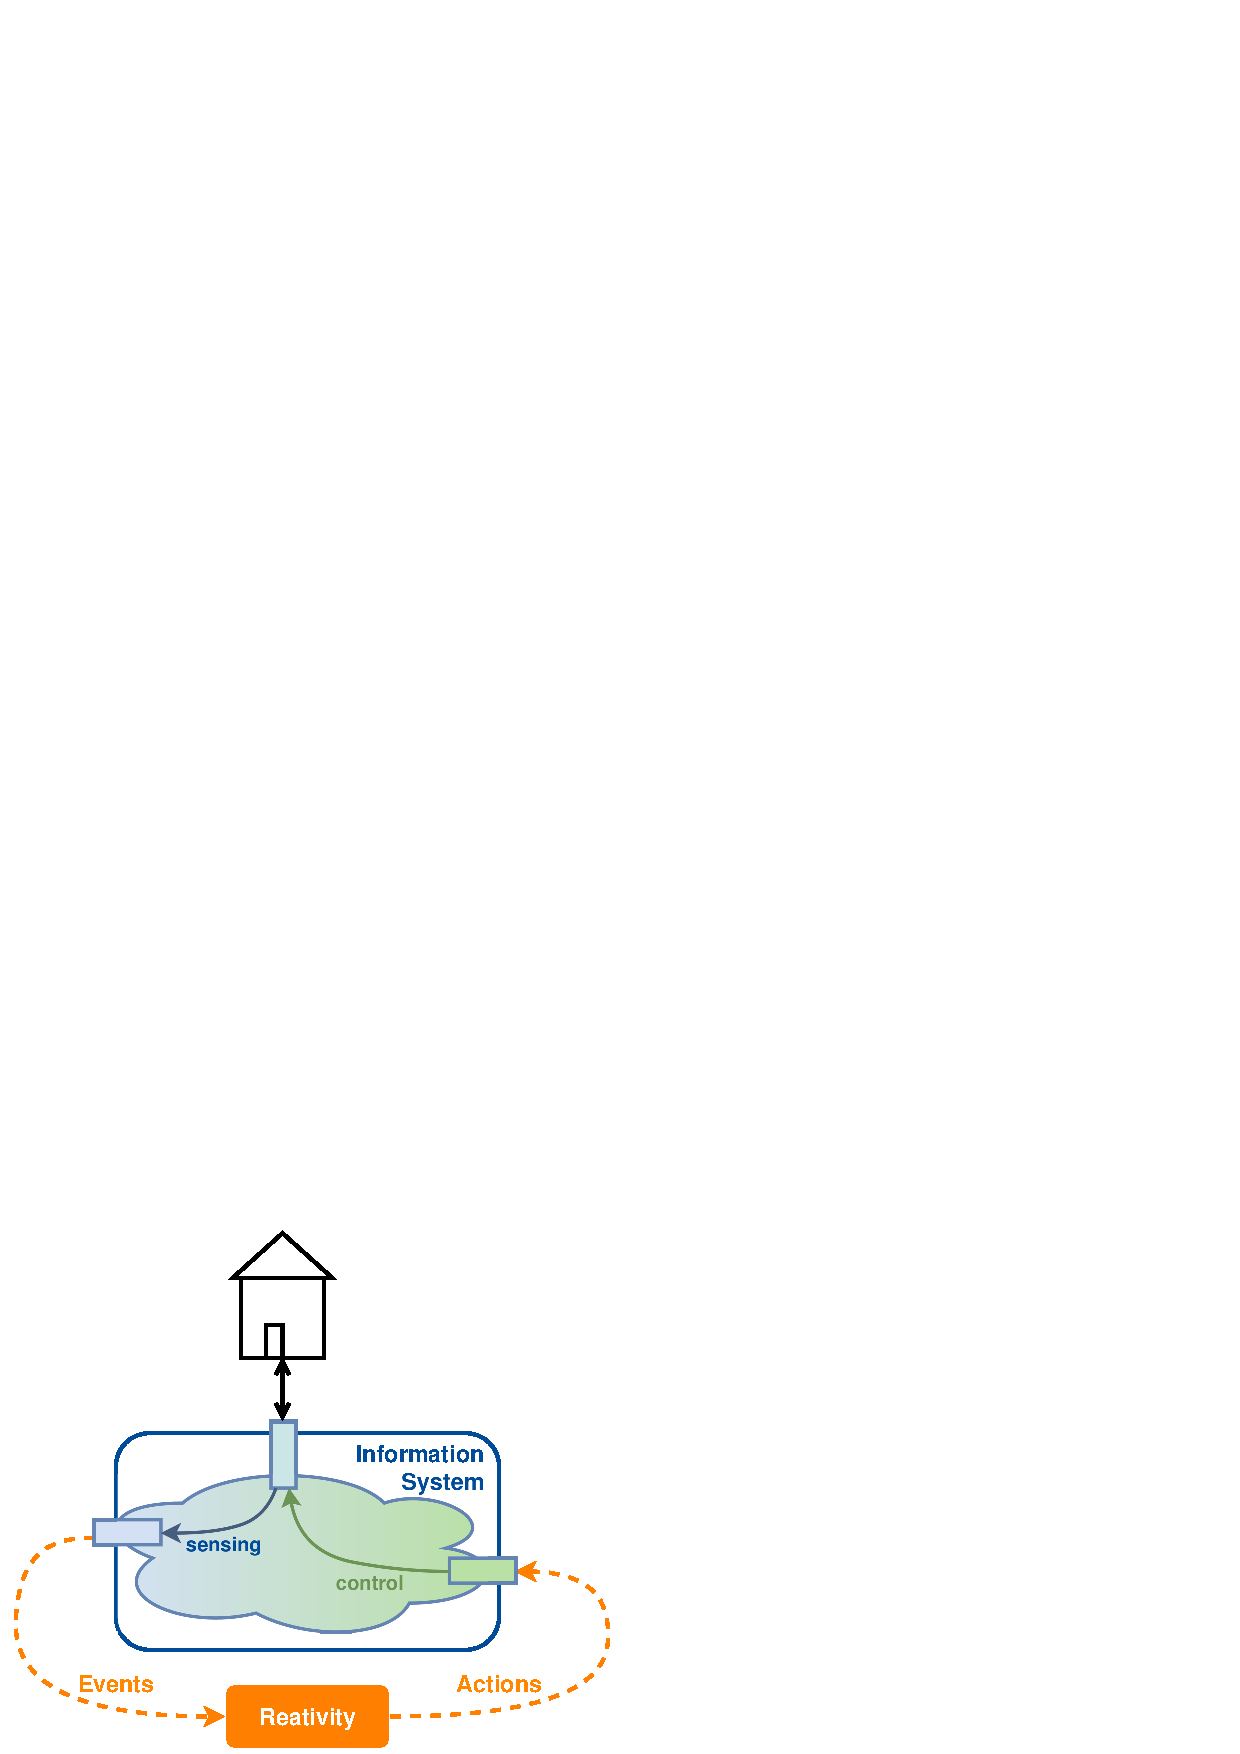
\includegraphics[width=0.6\textwidth]{figures/InformationSystemWoT}
  \caption{Conceptual Model for Reactive Information Systems and their Services}
  \label{fig:InformationSystemWoT}
\end{figure}

Since we have all the parts to access \textrm{\glspl{infosystem}} over their services, we are now able to define a \textrm{Rule Engine} that orchestrates them in a reactive way.
We have shown in the last chapter that \textrm{\acrshort{eca}} rules consist of three parts; an event to be recognized, conditions to be evaluated on the event and actions to be executed if an event triggers the rule through valid conditions.
We have also seen that virtual events have an implicit parameter which is the event name, thus this is the one that is referred to in the event part of a rule.
If an event name, of an event entering the \textrm{Rule Engine}, is detected in a predefined rule, the engine compares the event against the conditions of that rule and if all conditions are met, dispatches the actions defined within the rule.
We introduced \textrm{\acrshort{xml}} and \textrm{\acrshort{json}} as common ways to communicate data between services in the Web.
Both data formats represent a tree structure of the transmitted data and this also what we expect for the explicit parameters in the events that go through our model.
We also assume that \textrm{Action Dispatcher} modules can be accessed through common function invocation syntax ( \texttt{actionFunction(param1, param2[, ...])} ) in order to dispatch a certain action to an \textrm{\gls{infosystem}}.
Through this we are able to define a rule language that uses tree node selectors in order to select explicit event parameters, which are then used to verify conditions and forwarded to \textrm{Action Dispatcher} modules as function parameters.

\subsection{Rule Language for Reactive Information Systems}

% TODO conditions with examples
% TODO Imposing Acitons
% since we model changes in the data of an information space as events and actions, depending on wheter it is a read or wrtie action, we can impose reactivity to information systems.



% RL <-> ECA
% TODO figure: ECA Schema
% TODO Figure: ECA in the distributed environemnt
% TODO figure: Rules (unions / objects / Rueckkoppelungen )
% TODO engine




Because of the heterogenous nature of the Web actions need to be abstracted
as long as we do not limit ourselves e.g for RESTful access to services



% % Regelimplementierungssprache
% \subsection{Conceptual Rule Language}
% Describe conceptual rule language
% ON (existing categories)
% IF (condition boundaries)
% DO (call to existing action modules with parameters)

% a lot possible, but dangerous.

% \begin{Verbatim}[fontsize=\small,commandchars=\\\{\}]
% \PY{k}{on} \PY{n}{mail}
% \PY{k}{if} \PY{n}{sender}\PY{o}{=}\PY{l+s+ss}{\PYZdq{}sender@mail.com\PYZdq{}}
% \PY{k}{do} \PY{n}{webapi}\PY{o}{\PYZhy{}}\PY{o}{\PYZgt{}}\PY{l+s+s2}{newcontent}\PY{p}{(}\PY{n}{subject}\PY{p}{)}
% \end{Verbatim}

% % TODO Define language with regular expression 
% % Programming language syntax is usually defined using a combination of regular expressions (for lexical structure) and Backus–Naur Form (for grammatical structure). Below is a simple grammar, based on Lisp:
% % expression ::= atom | list
% % atom       ::= number | symbol
% % number     ::= [+-]?['0'-'9']+
% % symbol     ::= ['A'-'Z''a'-'z'].*
% % list       ::= '(' expression* ')'
% \begin{lstlisting}[language=OwnRule,caption=Conceptual ECA Rule Language Syntax]
% expression  ::= 'on ' event ' if ' conditions ' do ' actions
% event       ::= symbol.*(' -> ' symbol.*)
% conditions  ::= 
% actions     ::= symbol*('('selector*')')
% symbol      ::= [A-Za-z0-9_-]+
% selector    ::= [#\{(symbol*?)\}]
% \end{lstlisting


% TODO Action Dispatcher
% Actions
% \begin{itemize}
%   \item Event Redirection
%   \item Event Enrichment
%   \item WebApp Actions
% \end{itemize}





% EARTH QUAKE example

% Different points on earth's surface would feel the earthquake, which originates from the same epicentre, at a different point in time with a different intensity.
% A Web event model of an earthquake would consist of a large number of identical \textrm{\textbf{ground-shake}} events that occur at different points in time and places.
% Therefore they would hold different spatial location informations and intensities.
% These events can be thought of as emitted into the Web by a seismometer sitting at the corresponding location.
% \begin{figure}[!ht]
%   \centering
%   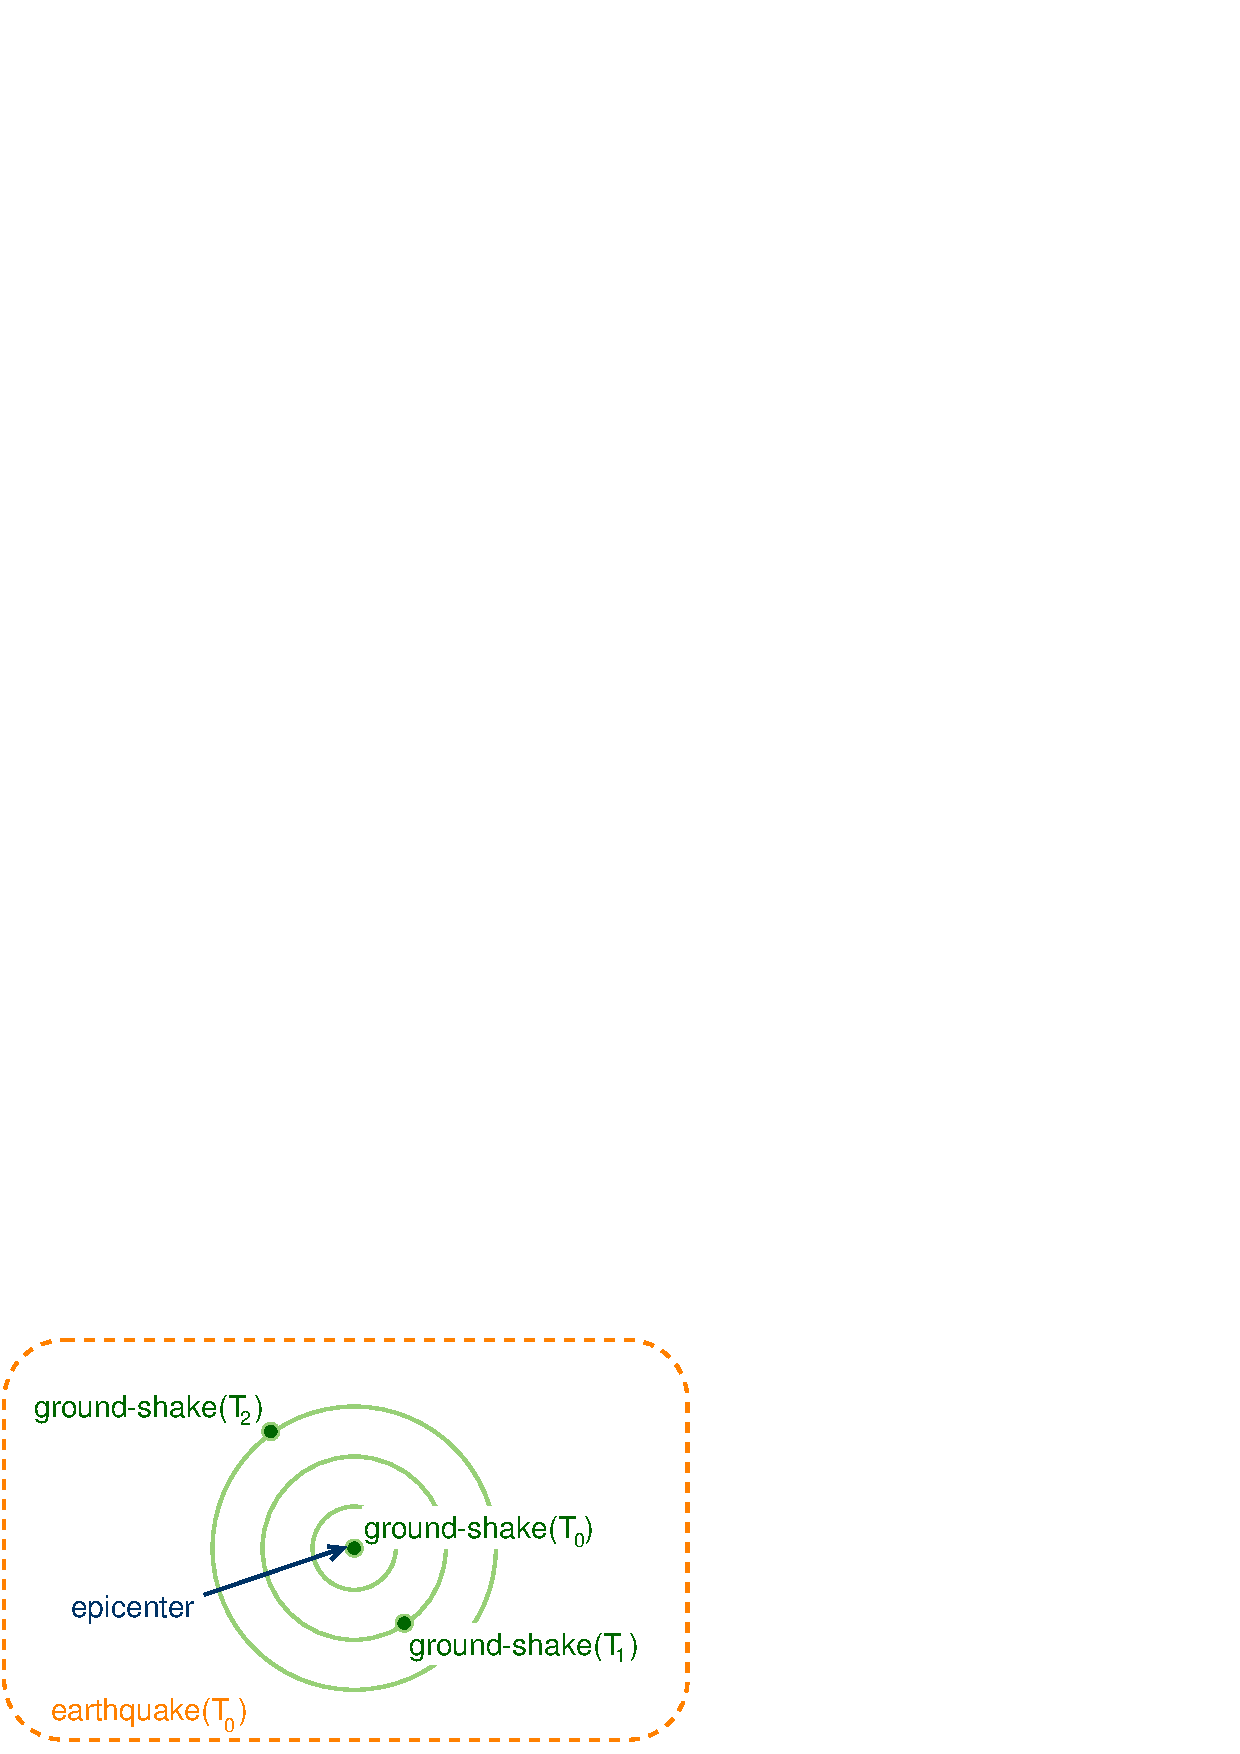
\includegraphics[width=0.6\textwidth]{figures/Earthquake}
%   \caption{Web Event Model of an Earthquake}
%   \label{fig:Earthquake}
% \end{figure}
% Within the Web, events lose their tight coupling to locations and retain only a time component.
% The event instances keep this information as descriptive metadata.
% A reactive system such as we envision it, could detect these \textrm{\textbf{ground-shake}} events and react on behalf of each one of them.
% Because of the Web's latency these events do most certainly not arrive at systems within the Web in the original order, in which they were triggered.
% They also do most likely not arrive in the exact same order for all systems.
% This leaves us with time as the only important factor left, to distinguish events from each other in the first place.
% To get an earthquake event out of all these ground shaking informations floating through the Web, somebody would need a reactive system that detects these events and assembles them into one earthquake event, together with a computed epicentre and magnitude.
% Such a system (we call it \textrm{\textbf{earthquake-tracker}}) would own an earthquake model that allows it to decide whether a \textrm{\textbf{ground-shake}} event belongs to one physical earthquake or to another one, depending on its spatial location information and the intensity at that point in time.
% It could then emit a more complex \textrm{\textbf{earthquake}} event (with epicentre and magnitude) that allows other systems to interpret this physical event and react on behalf of it.

% Let's take another system that reacts on a physical earthquake.
% It is now left with a multitude of different options on how to react.
% It could only react on the \textrm{\textbf{earthquake}} event which is coming from the system above (\textrm{\textbf{earthquake-tracker}}) that applies its earthquake model to the incoming \textrm{\textbf{ground-shake}} events.
% But how long will it take for this system to deploy its \textrm{\textbf{earthquake}} event?
% Eventually it waits for one round-trip of a seismic wave around the world, which takes approximately half an hour.
% What if it waits two or three round-trip times in order to collect more accurate data?
% And what if our new system wants to react as fast as possible in order to warn people all around the world.
% It would then need to react on a small subset of the \textrm{\textbf{ground-shake}} events in order to quickly identify a real earthquake and take measurements, e.g. immediately send out text messages to people, or to deploy yet another ( this time \textrm{\textbf{earthquake-alert}}) event into the Web's \textrm{\gls{infospace}}.
% This relatively simple example discloses the complex nature of event-driven systems, but also their high flexibility and fine grained tuning possibilities.

	\chapter{Scope of Applicability}
% informal description of target / story -> show that it makes sense
% Use Cases, not concrete

	

\chapter{Prototype System}
We have so far introduced our conceptual model for reactive \textrm{\glspl{infosystem}} and their Services and some example use cases to point out what would be possible with our model.
In this chapter we present our proof of concept prototype system, which has a focus on the Web as its \textrm{\gls{infospace}}.
We will then introduce our \textrm{\acrshort{eca}} rule language, which gives all the necessary power over our prototype system and which can be directly translated into the internal rules representation.



\section{Architecture}
The prototype system is the adoption of our conceptual model for reactive \textrm{\glspl{infosystem}} and their services to the Web.
The Web consists of many \textrm{\glspl{infosystem}} and because of its \textrm{\acrlong{soa}} it can be seen as one large \textrm{\gls{infosystem}}, therefore we can impose reactivity on the Web.
Since communication over services in the Web is often latency driven, we came to the conclusion that asynchronous communication and therefore scalability should be attributes our prototype system has to support natively.
Another aspect to be regarded for the architectural decision was how the rules are going to be represented internally.
We introduced \textrm{\acrshort{xml}} and \textrm{\acrshort{json}} as common ways to communicate data between services on the Web.
Both formats represent data in a tree structure, and this is also what we decided to assume for the explicit parameters in the events that will enter our prototype.
Together with the requirement of native support for an \textrm{\acrlong{eda} (\acrshort{eda})} our decision was to build upon the recent adoption of \textrm{JavaScript} to application development through \textrm{Node.js}\footnote{http://nodejs.org/} and its human-readable \textrm{\acrshort{json}} communication format.

The prototype system consists of several modules, shown in Figure \ref{fig:Architecture}, which we are going to introduce within this section:
\begin{itemize}
	\item \textbf{\textrm{Poller}:} Loads \textrm{Event Trigger} modules and forwards events coming from them to the \textrm{Event Queue}. \textrm{Event Trigger} modules poll for changes in the Web and transform them into events. 
	\item \textbf{\textrm{\gls{webhook} Listener}:} Listens on active \textrm{\gls{webhook}} for events and forwards them to the \textrm{Event Queue}.
	\item \textbf{\textrm{Event Queue}:} Buffers events for the case of an overly busy \textrm{Rule Engine}. 
	\item \textbf{\textrm{Rules Engine}:} Picks an event from the \textrm{Event Queue} whenever there is one and it is idle. 
	\item \textbf{\textrm{User Request Handler}:} The user interface modules to administrate \textrm{Event Triggers}, \textrm{\gls{webhook}}, \textrm{Rules} and \textrm{Action Dispatchers}.
\end{itemize}

When started, the prototype system loads persisted \textrm{\gls{webhook}} and begins to listen for new events on them.
The \textrm{Rule Engine} then loads all persisted rules and for each rule it loads the required \textrm{Action Dispatchers} and notifies the \textrm{Poller} about the new rule, which in turn loads an \textrm{Event Trigger} if required.
The prototype is now up and running and accepts administration requests for \textrm{Event Triggers}, \textrm{\gls{webhook}}, \textrm{Rules} and \textrm{Action Dispatchers}.
Whenever a rule is created or updated, the \textrm{Poller} and \textrm{Rule Engine} load required \textrm{Event Triggers} or \textrm{Action Dispatchers}.

\begin{figure}[!ht]
	\centering
  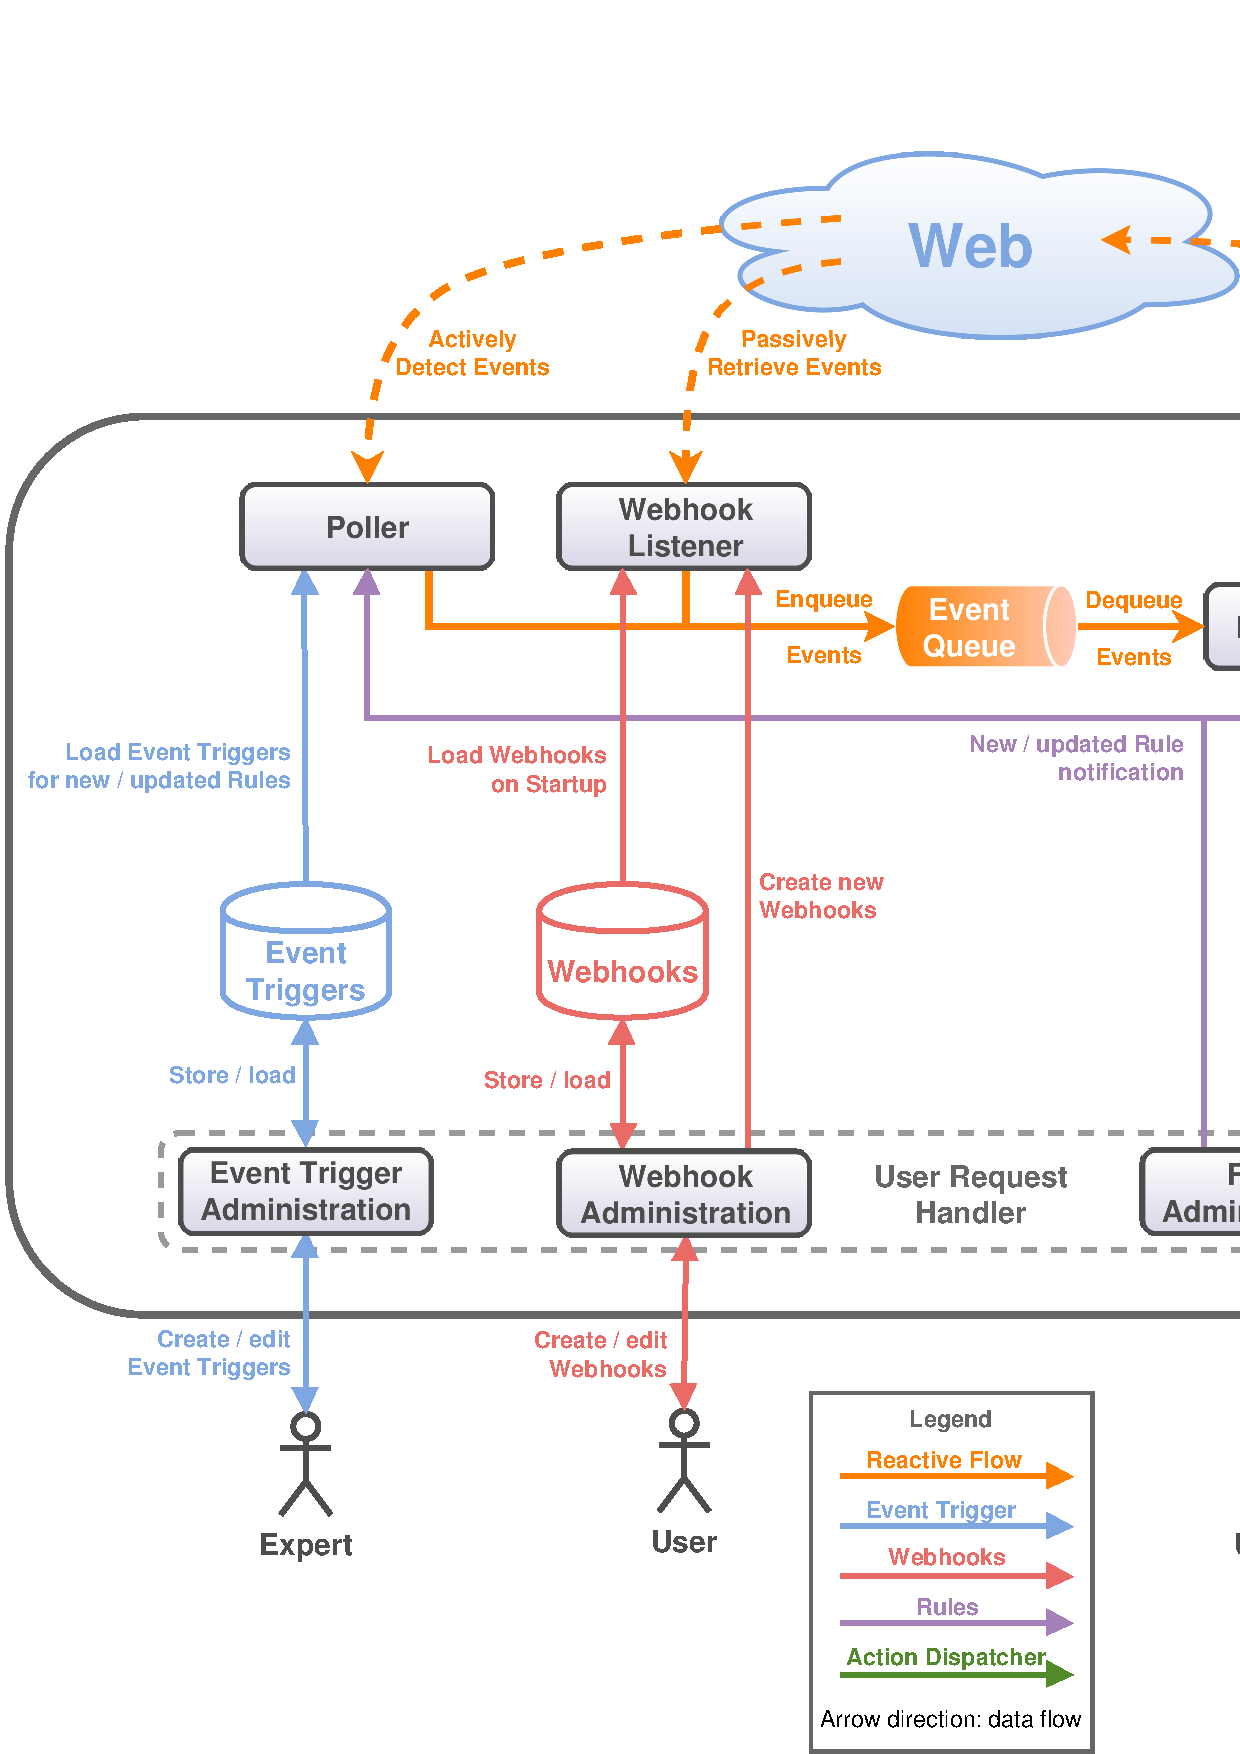
\includegraphics[width=\textwidth]{figures/Architecture_Final}
	\caption{Prototype System Architecture}
	\label{fig:Architecture}
\end{figure}



\subsection{Data Structure for Event Parameters}
Events in our prototype system are internally represented as tree structures in \textrm{\acrshort{json}} format.
The \textrm{\acrshort{json}} format builds on two data structures:
\begin{itemize}
	\item Objects: Unordered collections of name/value pairs wrapped in curly brackets \texttt{\{ \}}, which can also be implemented as a hash map, dictionary or struct in other languages.
	\item Arrays: Ordered lists of values wrapped in brackets \texttt{[ ]}, which can also be implemented as a record, vector or list in other languages.
\end{itemize}
A value can be an object or an array, but also a unicode string, a number, a boolean value or null.
This allows for any arbitrary depth and chaining of the supported data representations.
It is a handy feature when we assume a tree structure for events in our prototype system since the selection of nodes in tree structures has been well studied and useful libraries exist.
\textrm{\acrshort{json}} formatted datastructures can easily be marshaled into one string and communicated to other applications without overhead
Also, they are natively supported within \textrm{JavaScript} programming code. 
\textrm{\acrshort{json}} can be implemented in virtually every programming language, therefore received a lot of attention and is supported by many \textrm{\glspl{webresource}} for communication.



\subsection{Dynamic Code Loading for Event Trigger and Action Dispatcher}
During our research we have seen many different \textrm{\glspl{webservice}} with thoroughly different requirements in terms of communication.
The cleanest category among them were the \textrm{\glspl{webapi}} with their \textrm{\acrshort{rest}}ful services.
And still, in many cases it is only possible to access data which does not refer to an event.
To detect a change in data over time we need to be able to store an earlier request and get the difference to the current request, which could then be transformed into a meaningful event.
The derivation of a meaningful event from data can be a complex task which requires certain operations, which underlines the need for powerful \textrm{Event Trigger} modules.
The complexity is even bigger for \textrm{Action Dispatcher} modules which alter data and require more complex communication to \textrm{\glspl{webservice}}.
For those reasons we made the decision to keep these modules flexible in terms of communication.
We also wanted to leave it open to expert users to encapsulate complicated logic into them for inexperienced users.
We modeled the \textrm{Event Trigger} and \textrm{Action Dispatcher} to be \textrm{JavaScript} code modules, which are created by expert users during runtime.
They are also loaded during runtime whenever an activated rule needs them.
These modules run in a sandbox and got only access to certain \textrm{JavaScript} libraries, which are provided by the owner of the system.
Through this it is possible to communicate with \textrm{\acrshort{rest}}ful \textrm{\glspl{webservice}} as well as with \textrm{\acrshort{soap}} \textrm{\glspl{webService}} or any other service that can be addressed through \textrm{JavaScript} libraries. 
Apart from those libraries there are two other important functions offered in both type of modules:
\begin{itemize}
	\item \textrm{log}: Will store log entries on a per rule base, wherever the instruction is met during execution of a module.
	The log can be seen by the user who chose the module to be part of a rule.
	\item \textrm{pushEvent}: This funciton is an important part of \textrm{Event Trigger} modules.
	It is responsible to push events into the prototype system. For \textrm{Action Dispatcher} modules this provides the possibility for loopback events.
\end{itemize}
Only functions which are attached to the \texttt{exports} property of the module are later accessible from the outside and can be selected as \textrm{Event Trigger} or \textrm{Action Dispatcher}.
The function arguments of, from outside visible, functions are identified by the according \textrm{User Request Handler} module and the user will be requested to provide values for all of them in order to activate the \textrm{Event Trigger} or \textrm{Action Dispatcher}.
For \textrm{Action Dispatchers} it is also possible to use event property selectors as arguments and thus allows the passing of event data to the \textrm{Action Dispatchers}.
Through the \texttt{pushEvent} function in the global scope of the modules, events can be pushed into the prototype system.

By using the expressiveness of \textrm{JavaScript} and some of its libraries, it is possible to access a large part of the existing \textrm{\glspl{infosystem}} and transform changes in their \textrm{\glspl{infospace}} into events and also to impose changes onto them as part of actions.
The power that can be expressed in those code modules needs to be controlled, and ca not be granted to anybody, thus we shield it through user access control, thus only allowing trusted users to write \textrm{Event Trigger} and \textrm{Action Dispatcher} code.



\subsection{Retrieving Events}
In the last chapters, we put emphasis on the two different ways how events can be retrieved from \textrm{\glspl{infosystem}}, i.e. actively pulling events, or passively retrieving them.
Some \textrm{\glspl{infosystem}} offer access to data that corresponds to events and can instantly be forwarded into the system.
But we have seen that there is need for the derivation of events from changes in data on the Web, therefore we need the \textrm{Event Trigger} modules.
But still, our vision is that of an optimal real-time reactive Web which means that all possible events are offered by all \textrm{\glspl{infosystem}}.
An interested remote entity could announce interest in a certain kind of events over a \textrm{\gls{webhook}} and would retrieve them in real-time.
For that reason we laid out our architecture for \textrm{\glspl{webhook}}, but still offer the \textrm{Event Trigger} modules to poll for events in the semi-static \textrm{\gls{www}}.
During prototype testing we focused mainly on server-sided \textrm{Web APIs}, but we also generated events from the browser and pushed them to our prototype system.
This was achieved with a library included in a sample webpage that pushed events to a \textrm{\gls{webhook}} of our prototype.
Since modern browsers support geo locating, we decided to let the client browser push the current position of the device to the \textrm{\gls{webhook}}.



\subsubsection{Polling with Event Triggers}
As we have pointed out before, \textrm{Event Trigger} modules are dynamic code modules with access to a set of predefined libraries.
The \textrm{Poller} loads \textrm{Event Trigger} modules whenever they are required in an active rule.
The user of the \textrm{Event Trigger} can choose a starting point and an interval for the polling to take place.
An example \textrm{\gls{webservice}} which offers polling for events is the \textrm{Email Yak}\footnote{http://www.emailyak.com/} \textrm{\gls{webapi}}, which responds with new emails when requested.
The code required to request the new mails from this service and forward them into the prototype system is quite short and shown in Listing \ref{lst:emailyak}.
For other services it can quickly get more complex, depending on how complicated a meaningful change detection is.
For better readability the code is written in \textrm{CoffeeScript}\footnote{http://coffeescript.org/}.
Only expert users are expected to store such a piece of code in our prototype, which enables inexperienced users to simply choose the \texttt{"EmailYak -> newMail"} \textrm{Event Trigger} for their rule.  
A great opportunity to access data from webpages via a \textrm{\gls{webapi}} is \textrm{Import.io}\footnote{https://import.io/}.
By browsing through the Web with the \textrm{Import.io} browser, it is possible to select certain parts from a webpage and store the selection as a mask.
Data is instantly extracted from the webpage, using the stored mask, when sending a request to their \textrm{\gls{webapi}} with the given mask id and the \textrm{\acrshort{uri}}.
This is a great tool for expert users to predefine desired data on webpages and then produce events out of an \textrm{Event Trigger} whenever there is a change in that data.
\begin{lstlisting}[float=h,label=lst:emailyak,language=CoffeeScript,caption=Event Trigger code to poll Email Yak RESTful Web service for new Mails; written in CoffeeScript]
url = "https://api.emailyak.com/v1/#{params.apikey}/json/get/new/email/"
exports.newMail = () ->
	needle.get url, ( err, resp, body ) ->
		if not err and resp.statusCode is 200
				pushEvent mail for mail in body.Emails
\end{lstlisting}



\subsubsection{\gls{webhook}}
As powerful as their ability to provide real-time notifications from remote \textrm{\glspl{webresource}} is, as simple are \textrm{\glspl{webhook}} to use.
In our prototype, users can create as many new \textrm{\gls{webhook}} as they like.
They only need to provide an event name which will be associated to the \textrm{\gls{webhook}}.
A new \textrm{\gls{webhook}} is created in the \textrm{\gls{webhook} Listener}, which from then on accepts events posted to it.
The \textrm{\gls{webhook} \acrshort{uri}} is always accessible to the user and can be placed at any desired \textrm{\gls{webhook}} in order to receive events from it.
Any \textrm{\gls{webresource}} that supports the concept of \textrm{\gls{webhook}} (e.g. \textrm{GitHub}\footnote{https://developer.github.com/\gls{webhook}/}) has a place to register the \textrm{\gls{webhook}} \textrm{\acrshort{uri}}.
Whenever a remote \textrm{\gls{webresource}} pushes an event to the \textrm{\gls{webhook}}, the user-defined event name is assigned as the implicit parameter of a freshly created internal event.
The whole incoming event body is added as explicit parameters to the internal event, which is forwarded to the \textrm{Event Queue}.



\subsection{Dispatching Actions}
\textrm{Action Dispatchers} are \textrm{JavaScript} code modules that can be created during runtime and loaded by the engine whenever a new rule requires them, much as the \textrm{Event Trigger} modules are loaded by the \textrm{Poller}.
Before actions can be used in a rule, an expert has to create them.
In our prototype system, \textrm{Action Dispatchers} use a library for \textrm{HTTP} communication which allows them to address a wide range of \textrm{\glspl{webresource}}.
\textrm{Action Dispatchers} can also push events back into the \textrm{Event Queue} which can be used to chain certain rules together.
Since \textrm{\glspl{webhook}} are an important part of our vision we also implemented an \textrm{Action Dispatcher} that delivers events to external \textrm{\gls{webhook}}.
\textrm{Action Dispatchers} need to have functions attached to their \texttt{exports} property so that they are visible from the outside and can be selected as actions, such as the \texttt{newContent} function in the example Listing \ref{lst:actionProBinder}.
\begin{lstlisting}[float=h,label=lst:actionProBinder,language=CoffeeScript,caption=Action Dispatcher code to store a new content on the ProBinder RESTful Web service; written in CoffeeScript]
urlService = 'https://probinder.com/service/'

requestService = ( args ) ->
  url = urlService + args.service + '/' + args.method
  needle.post url, args.data

exports.newContent = ( companyId, contextId, content ) ->
  requestService
    service: 'content'
    method: 'save'
    data:
      companyId: companyId
      context: contextId
      text: content
\end{lstlisting}



\subsection{\acrshort{eca} Rules in the Rule Engine}
While a car engine converts potential energy into mechanical work, our \textrm{Rule Engine} converts events into changes in \textrm{\glspl{infosystem}}.
We have introduced \textrm{\acrshort{eca}} rules as sufficient approach to impose reactivity on systems and adopted the \textrm{\acrshort{eca}} paradigm for our conceptual model.
For our prototype this means that the \textrm{Rule Engine} requires user-defined \textrm{\acrshort{eca}} rules which are compared against incoming events.
The \textrm{Rules Administration} within the \textrm{User Request Handler} notifies the \textrm{Rules Engine} about new or updated rules from the user, which then in turn loads required \textrm{Action Dispatcher} modules.
For each event in the \textrm{Event Queue}, the engine checks it against its stored \textrm{\acrshort{eca}} rules and dispatches actions whenever the event conforms to the rule's condition part.
The three parts of an \textrm{\acrshort{eca}} rule have the following requirements in our prototype system:
\begin{itemize}
	\item Event name: Any arbitrary Unicode string, can refer to the name of an \textrm{Event Trigger} or a \textrm{\gls{webhook}}, but also to a custom loopback event.
	\item Conditions: Zero or more instructions to be evaluated against an event. Requires a selector for a node in the tree structure of the event, a comparison operator ($<$, $<=$, $>$, $>=$, $==$, $!=$ or $instr$) and a value.
	\item Action Dispatchers: A list of \textrm{Action Dispatchers} to be invoked if all conditions of the given event evaluate to true. We assume that invocations can be expressed using common function invocation syntax ( i.e. \texttt{actionFunction(param1, param2[, ...])} ) in order to dispatch an action.
\end{itemize}
A valid rule in the internal \textrm{\acrshort{json}} representation is shown in Listing \ref{lst:rulejson}, where we used the predefined \textrm{EmailYak Action Dispatcher} to send a mail to an interested person whenever news about soccer are detected.

\subsubsection{Parameter Selectors for Events}
Tree node selectors for event parameters are used in conditions to select a parameter which is evaluated.
The selectors can also be used to pass event parameters as arguments to the \textrm{Action Dispatchers}.
Event tree node selectors for \textrm{Action Dispatcher} arguments are defined by wrapping them into curly brackets and prepended with a hash: \texttt{"\#\{ [selector] \}"}.
Since an existing \textrm{JavaScript} library\footnote{https://github.com/harthur/js-select} is used to find event parameters with selectors, the following selectors are available\footnote{Explanations taken from http://jsonselect.org/, which is used by js-select}:
\begin{itemize}
	\item \textrm{\textbf{* :}}	Any node
	\item \textrm{\textbf{T :}}	A node of type T, where T is one string, number, object, array, boolean, or null
	\item \textrm{\textbf{T.key :}}	A node of type T which is the child of an object and is the value its parents key property
	\item \textrm{\textbf{T:root :}}	A node of type T which is the root of the JSON document
	\item \textrm{\textbf{T:nth-child(n) :}}	A node of type T which is the nth child of an array parent
	\item \textrm{\textbf{T:nth-last-child(n) :}}	A node of type T which is the nth child of an array parent counting from the end
	\item \textrm{\textbf{T:first-child :}}	A node of type T which is the first child of an array parent (equivalent to T:nth-child(1)
	\item \textrm{\textbf{T:last-child :}}	A node of type T which is the last child of an array parent (equivalent to T:nth-last-child(1)
	\item \textrm{\textbf{T:only-child :}}	A node of type T which is the only child of an array parent
	\item \textrm{\textbf{T U :}}	A node of type U with an ancestor of type T
	\item \textrm{\textbf{T $>$ U :}}	A node of type U with a parent of type T
	\item \textrm{\textbf{T $\sim$ U :}}	A node of type U with a sibling of type T
	\item \textrm{\textbf{S1, S2 :}}	Any node which matches either selector S1 or S2
	\item \textrm{\textbf{T:has(S) :}}	A node of type T which has a child node satisfying the selector S
	\item \textrm{\textbf{T:val(V) :}}	A node of type T with a value that is equal to V
	\item \textrm{\textbf{T:contains(S) :}}	A node of type T with a string value contains the substring
\end{itemize}
\begin{Verbatim}[samepage=true,frame=single,fontsize=\footnotesize,commandchars=\\\{\},numbers=left,firstnumber=1,stepnumber=1,xleftmargin
=.3in]
\PY{p}{\PYZob{}}
  \PY{n+nt}{\PYZdq{}eventname\PYZdq{}}\PY{p}{:} \PY{l+s+s2}{\PYZdq{}news\PYZdq{}}\PY{p}{,}
  \PY{n+nt}{\PYZdq{}conditions\PYZdq{}}\PY{p}{:} \PY{p}{[}
    \PY{p}{\PYZob{}}
      \PY{n+nt}{\PYZdq{}selector\PYZdq{}}\PY{p}{:} \PY{l+s+s2}{\PYZdq{}.categories\PYZdq{}}\PY{p}{,}
      \PY{n+nt}{\PYZdq{}operator\PYZdq{}}\PY{p}{:} \PY{l+s+s2}{\PYZdq{}instr\PYZdq{}}\PY{p}{,}
      \PY{n+nt}{\PYZdq{}compare\PYZdq{}}\PY{p}{:} \PY{l+s+s2}{\PYZdq{}soccer\PYZdq{}}
    \PY{p}{\PYZcb{}}
  \PY{p}{]}\PY{p}{,}
  \PY{n+nt}{\PYZdq{}actions\PYZdq{}}\PY{p}{:}\PY{p}{[}
    \PY{l+s+s2}{\PYZdq{}EmailYak\PYZhy{}\PYZgt{}sendMail(\PYZbs{}\PYZdq{}fan@soccer.com\PYZbs{}\PYZdq{},\PYZbs{}\PYZdq{}News about soccer!\PYZbs{}\PYZdq{},\PYZbs{}\PYZdq{}\PYZsh{}\PYZob{} .body \PYZcb{}\PYZbs{}\PYZdq{})\PYZdq{}}
  \PY{p}{]}
\PY{p}{\PYZcb{}}
\end{Verbatim}
\vspace{-0.7cm}
\begin{lstlisting}[float=h,frame=no,label=lst:rulejson,caption=Rule Example expressed in \textrm{\acrshort{json}}]
\end{lstlisting}

\section{A Rule Language for the Prototype System}
So far, we introduced the internal representation of the \textrm{\acrshort{eca}} rule language used in our prototype system.
For human readability and more intuitive writing, they can be transformed into a phrase representation, through which Listing \ref{lst:rulejson} would be written as shown in Listing \ref{lst:exampleRulePhrase}.
Our language is descriptive and flexible in terms of the \textrm{Event Trigger} and \textrm{Action Dispatcher} modules.
Another important flexible factor is the mapping of event properties to the \textrm{Action Dispatchers}.
To write a rule it requires a priori information from the \textrm{Event Trigger} and \textrm{Action Dispatcher} modules, but we believe this can be offered intuitively to the user through today's \textrm{\glspl{webapplication}}.
Listing \ref{lst:exampleRulePhrase} shows an example phrase of our envisioned rule language where the retrieval of a new mail will be checked for soccer news and, if confirmed, the mail body will be forwarded to an interested person.
The Extended Backus-Naur Form for the prototype rule language syntax is shown in Listing \ref{lst:backusnaur}.

\begin{lstlisting}[float=h,language=OwnRule,label={lst:exampleRulePhrase},caption=Example Phrase in Prototype Rule Language]
ON news
IF ".categories" instr "soccer"
DO EmailYak->sendMail("fan@soccer.com","News about soccer!","#{ .body }")
\end{lstlisting}

\begin{lstlisting}[float=h,language=OwnRule,label={lst:backusnaur},caption={Extended Backus-Naur Form of Prototype Rule Language Syntax}]
expression  ::= "ON " event " IF " conditions " DO " actions
event       ::= word* ("->" word+)?
conditions  ::= condition (" AND " condition)*
condition   ::= string operator "'" string "'"
operator    ::= (" < "|" <= "|" > "|" >= "|" == "|" != "|" instr ")
actions     ::= action (", " action)*
action      ::= word* "(" (argument ("," argument)*)? ")"
argument    ::= "'" selstring "'"
selstring   ::= (word|selector|" ")
selector    ::= "#{" string "}"
string      ::= (word|special|" ")*
special     ::= [():.*>~,]
word        ::= [A-Za-z0-9_-]+
\end{lstlisting}



\section{Prototype Use Case Implementations}
In the previous chapter we listed use cases for our conceptual model.
In this chapter we introduce use cases that were implemented in our prototype system in order to impose reactivity on the \textrm{\gls{web}}.


\subsection{Detecting responding Computers}
In our department building, one office is located on the other side of the floor and the elevator is right in the middle of it.
This resulted in one person frequently missing the coffee break, because everybody was always in a lively discussion towards the elevator and forgot about him.
Thus he sat up a network scanner that pinged the department's \textrm{Internet Protocol (IP)} range in the morning and pushed the results as events into the system.
Through this he was able to set up a rule that, if more than 42 pings were returned, the system automatically deployed an email invitation to the group, suggesting a coffee break.
The network scanner (code in Appendix \ref{lst:eventproducer}) was implemented as external \textrm{\gls{infosystem}} which pushed the ping results as event over a \textrm{\gls{webhook}}.
The rule is shown in Listing \ref{lst:ruleCoffeeBreak} and the corresponding simplified \textrm{Action Dispatcher} is shown in Listing \ref{lst:adEmailYak}.

\begin{Verbatim}[samepage=true,frame=single,fontsize=\footnotesize,commandchars=\\\{\},numbers=left,firstnumber=1,stepnumber=1,xleftmargin
=.3in]
\PY{p}{\PYZob{}}
  \PY{n+nt}{\PYZdq{}eventname\PYZdq{}}\PY{p}{:} \PY{l+s+s2}{\PYZdq{}uptimestatistics\PYZdq{}}\PY{p}{,}
  \PY{n+nt}{\PYZdq{}conditions\PYZdq{}}\PY{p}{:} \PY{p}{[}
    \PY{p}{\PYZob{}}
      \PY{n+nt}{\PYZdq{}selector\PYZdq{}}\PY{p}{:} \PY{l+s+s2}{\PYZdq{}.currentlyon\PYZdq{}}\PY{p}{,}
      \PY{n+nt}{\PYZdq{}operator\PYZdq{}}\PY{p}{:} \PY{l+s+s2}{\PYZdq{}\PYZgt{}\PYZdq{}}\PY{p}{,}
      \PY{n+nt}{\PYZdq{}compare\PYZdq{}}\PY{p}{:} \PY{l+m+mi}{42}
    \PY{p}{\PYZcb{}}
  \PY{p}{]}\PY{p}{,}
  \PY{n+nt}{\PYZdq{}actions\PYZdq{}}\PY{p}{:} \PY{p}{[}
    \PY{l+s+s2}{\PYZdq{}EMailYak \PYZhy{}\PYZgt{} sendMail(\PYZbs{}\PYZdq{}eca\PYZhy{}engine@mscliveweb.simpleyak.com\PYZbs{}\PYZdq{},[usermaillist],}
\PY{l+s+s2}{      \PYZbs{}\PYZdq{}Coffee Break!\PYZbs{}\PYZdq{},\PYZbs{}\PYZdq{}Let\PYZsq{}s go for a coffee at 10!\PYZbs{}\PYZdq{})\PYZdq{}}
  \PY{p}{]}
\PY{p}{\PYZcb{}}
\end{Verbatim}
\vspace{-0.7cm}
\begin{lstlisting}[float=h,language=OwnRule,caption={Rule; Coffee Break Invitation},label={lst:ruleCoffeeBreak},frame=no]
\end{lstlisting}

\begin{lstlisting}[float=h,language=CoffeeScript,caption={Action Dispatcher; EMailYak, in CoffeeScript},label={lst:adEmailYak}]
url = 'https://api.emailyak.com/v1/'+params.apikey+'/json/send/email/'

exports.sendMail = ( sender, receipient, subject, content ) ->
	data =
		FromAddress: sender
		ToAddress: receipient
		Subject: subject
		TextBody: content
	needle.post url, data, json: true
\end{lstlisting}


\subsection{Webpage Diff}




\subsection{Enhance Existing Web App}

\begin{lstlisting}[float=h,language=OwnRule,label={lst:RulePhraseAnnotate},caption=Rule Phrase for ProBinder Annotations]
ON ProBinder->unreadContent
IF "#{ .context .id }" == 18749
DO ProBinder->annotateTagEntries("#{ .id }"),
	 ProBinder->setRead("#{ .id }")
\end{lstlisting}


% on ProBinder->unreadContent
% if "#{ .context .id }" == 18749
% do "ProBinder -> annotateTagEntries(\"#{ .id }\")",
% 	 "ProBinder -> setRead(\"#{ .id }\")"
   

\subsection{Real-time Reactive Messenger}





% During our research we found a troublesome server room that made us develop a rule towards exposition of the \textrm{\gls{webofthings}}.
% This server room suffered from a defective cooling system which lead to a drastic increase of temperature in certain circumstances.
% As a consequence certain server automatically shut themselves down as safety measurements.
% In order to support the administrator we sat up 
% As a very quick fix to inform certain administrators about the shutdown of their server, we started pinging these servers and pushed the results int

\subsection{Page Rank of Webpage changes}


% Real-time reactive Web over \gls{webhook} -> instant messaging


% {
%     "dominic": {
%         "SOAP test": "{\"id\":\"SOAP test\",\"eventtype\":\"Custom Event\",\"eventname\":\"button-click\",\"conditions\":[],\"actions\":[\"SOAP -> convertCelsiusToFahrenheit\"]}",
%         "Presentation to Pushover": "{\"id\":\"Presentation to Pushover\",\"eventtype\":\"Custom Event\",\"eventname\":\"pushover\",\"conditions\":[],\"actions\":[\"Pushover -> broadcast\"]}",
%         "ProBinder Service Test: FAIL": "{\"id\":\"ProBinder Service Test: FAIL\",\"eventtype\":\"Custom Event\",\"eventname\":\"ProBinderServiceTest\",\"conditions\":[{\"selector\":\".success\",\"type\":\"bool\",\"operator\":\"==\",\"compare\":false}],\"actions\":[\"Pushover -> broadcast\",\"EMailYak -> sendMail\"]}",
%         "ProBinder Service Test": "{\"id\":\"ProBinder Service Test\",\"eventtype\":\"Event Poller\",\"eventname\":\"ProBinder Service Test -> testProBinder\",\"eventstart\":\"2014-05-20T13:00:00.000Z\",\"eventinterval\":120,\"conditions\":[],\"actions\":[\"System -> pushEvent\"],\"timestamp\":\"2014-05-20T11:51:46.307Z\"}",
%         "'button-click' Rule": "{\"id\":\"'button-click' Rule\",\"eventtype\":\"Custom Event\",\"eventname\":\"button-click\",\"conditions\":[],\"actions\":[\"Pushover -> broadcast\"]}",
%         "ProBinder annotate tags": "{\"id\":\"ProBinder annotate tags\",\"eventtype\":\"Event Poller\",\"eventname\":\"ProBinder -> unreadContent\",\"eventstart\":\"2014-05-20T19:11:00.000Z\",\"eventinterval\":1,\"conditions\":[],\"actions\":[\"ProBinder -> annotateTagEntries\",\"ProBinder -> setRead\"],\"timestamp\":\"2014-05-20T19:10:10.951Z\"}",
%         "Coffee Break": "{\"id\":\"Coffee Break\",\"eventtype\":\"Custom Event\",\"eventname\":\"uptimestatistics\",\"conditions\":[{\"selector\":\".currentlyon\",\"type\":\"value\",\"operator\":\">\",\"compare\":42}],\"actions\":[\"EMailYak -> sendMail\"]}",
%         "ProBinder Service Test: Logging": "{\"id\":\"ProBinder Service Test: Logging\",\"eventtype\":\"Custom Event\",\"eventname\":\"ProBinderServiceTest\",\"conditions\":[],\"actions\":[\"ProBinder -> newContent\"]}"
%     }
% }

\begin{figure}[!ht]
	\centering
  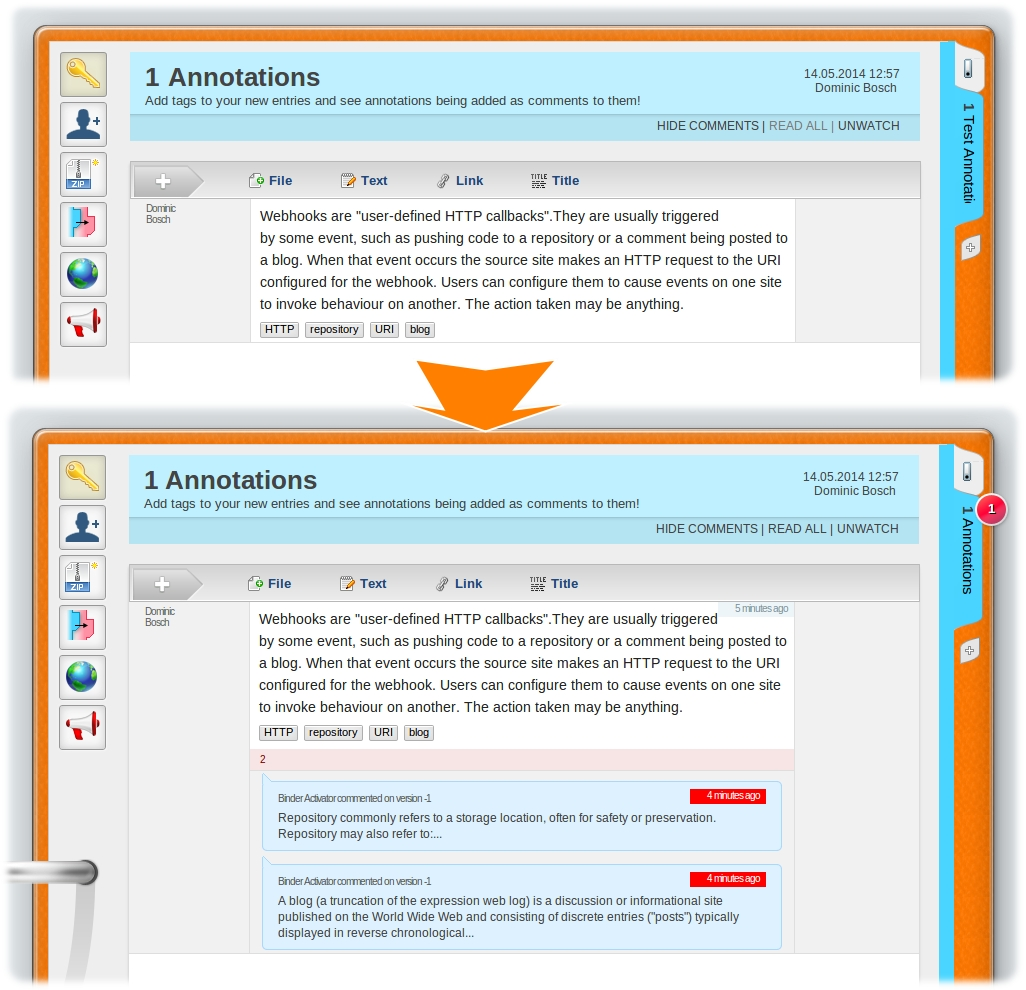
\includegraphics[width=\textwidth]{figures/UC_Binder_Annotations}
	\caption{UC Binder Annotation}
	\label{fig:UC_Binder_Annotations}
\end{figure}

\section{Web Application Development}
% Why JS, why was not it used up to now? is it used now?

% My guess is that Node is encouraging good programmer practices in terms of scalability, and Java less so. In other words, programmers probably have to work less hard to avoid bad scalability bottlenecks in Node than in Java.

% By incorporating JavaScript’s asynchronous design
% of callback functions into their architecture, locking situations are basically
% omitted. Thus it is a highly-scalable, asynchronous, event-driven architec-
% ture which found its acceptance in the open-source comunity as well as for
% enterprises.
% The package manager npm can be used to maintain dependencies of a
% custom node.js module to other modules. This helpful feature ensures that
% everybody working with the user-defined module uses the same external
% modules and the respective versions. Also project repositories do not need
% to store the dependent libraries through this mechanism, thus saving space


% full stack development 


% TODO why JS. JSON as first advantage (http://www.toptal.com/nodejs/why-the-hell-would-i-use-node-js)
% advantage for network applications with several concurrent connections
% not as client-server used as intented but as serverserver com since we also expect several connections simultanously under load.
% But also, we adopt the non-blocking nature of JS that is used for node's optimal communication, in order to implement our enigne in a non blocking way, thus allowing to load code and fire callback function in modules whenever they are required!
% http://ariya.ofilabs.com/2012/07/lazy-parsing-in-javascript-engines.html
% Optimization of special case if ( before function {immediately-invoked function expression (IIFE)}, do rela parsing, else lazy parsing
% Difference between context and scope. scope unique to each invocation, context is 'this', owner of currently executing code.
% .call, .apply 
% TODO we should use .bind for persistence.coffee's functions ....

%In JavaScript, functions are first-class objects, i.e. they are objects and can be manipulated and passed around just like any other object. Specifically, they are Function objects. -> https://developer.mozilla.org/en/docs/Web/JavaScript/Reference/Functions_and_function_scope
% Since each call provides potentially different arguments, a new closure is created for each call to outside. The memory can be freed only when the returned inside is no longer accessible

% The definitive guide: This combination of a function object and a scope (a set of variable bindings) in which the function’s variables are resolved is called a closure in the computer science literature.4
% This is an old term that refers to the fact that the function’s variables have bindings in the scope chain and that therefore the function is “closed over” its variables.



% Umgang mit der Zukunft
% Callback
\subsection{Callback Functions \& Asynchronous Closures}
% JAva futures? objekte für resultate sammeln
% Closures are functions that refer to independent (free) variables. 

Often, optimization approaches and programming language concepts require special attention to avoid common pitfalls.
When closures are used as asynchronous functions, developers need to be very careful not to end up with race conditions.


Looking at an example of sequential code execution in Figure~\ref{fig:Closures_Synchronous}, we see that function execution of \texttt{fA} is halted until function \texttt{fB} is finished.
If \texttt{fB} happens to be a latency-driven I/O operation the completion of \texttt{fA} could be deferred for a relatively long time.
While the application waits for the completion of the I/O operation, some remaining operations in \texttt{fA} could eventually already be executed without causing any race conditions.
\begin{figure}[!ht]
	\centering
  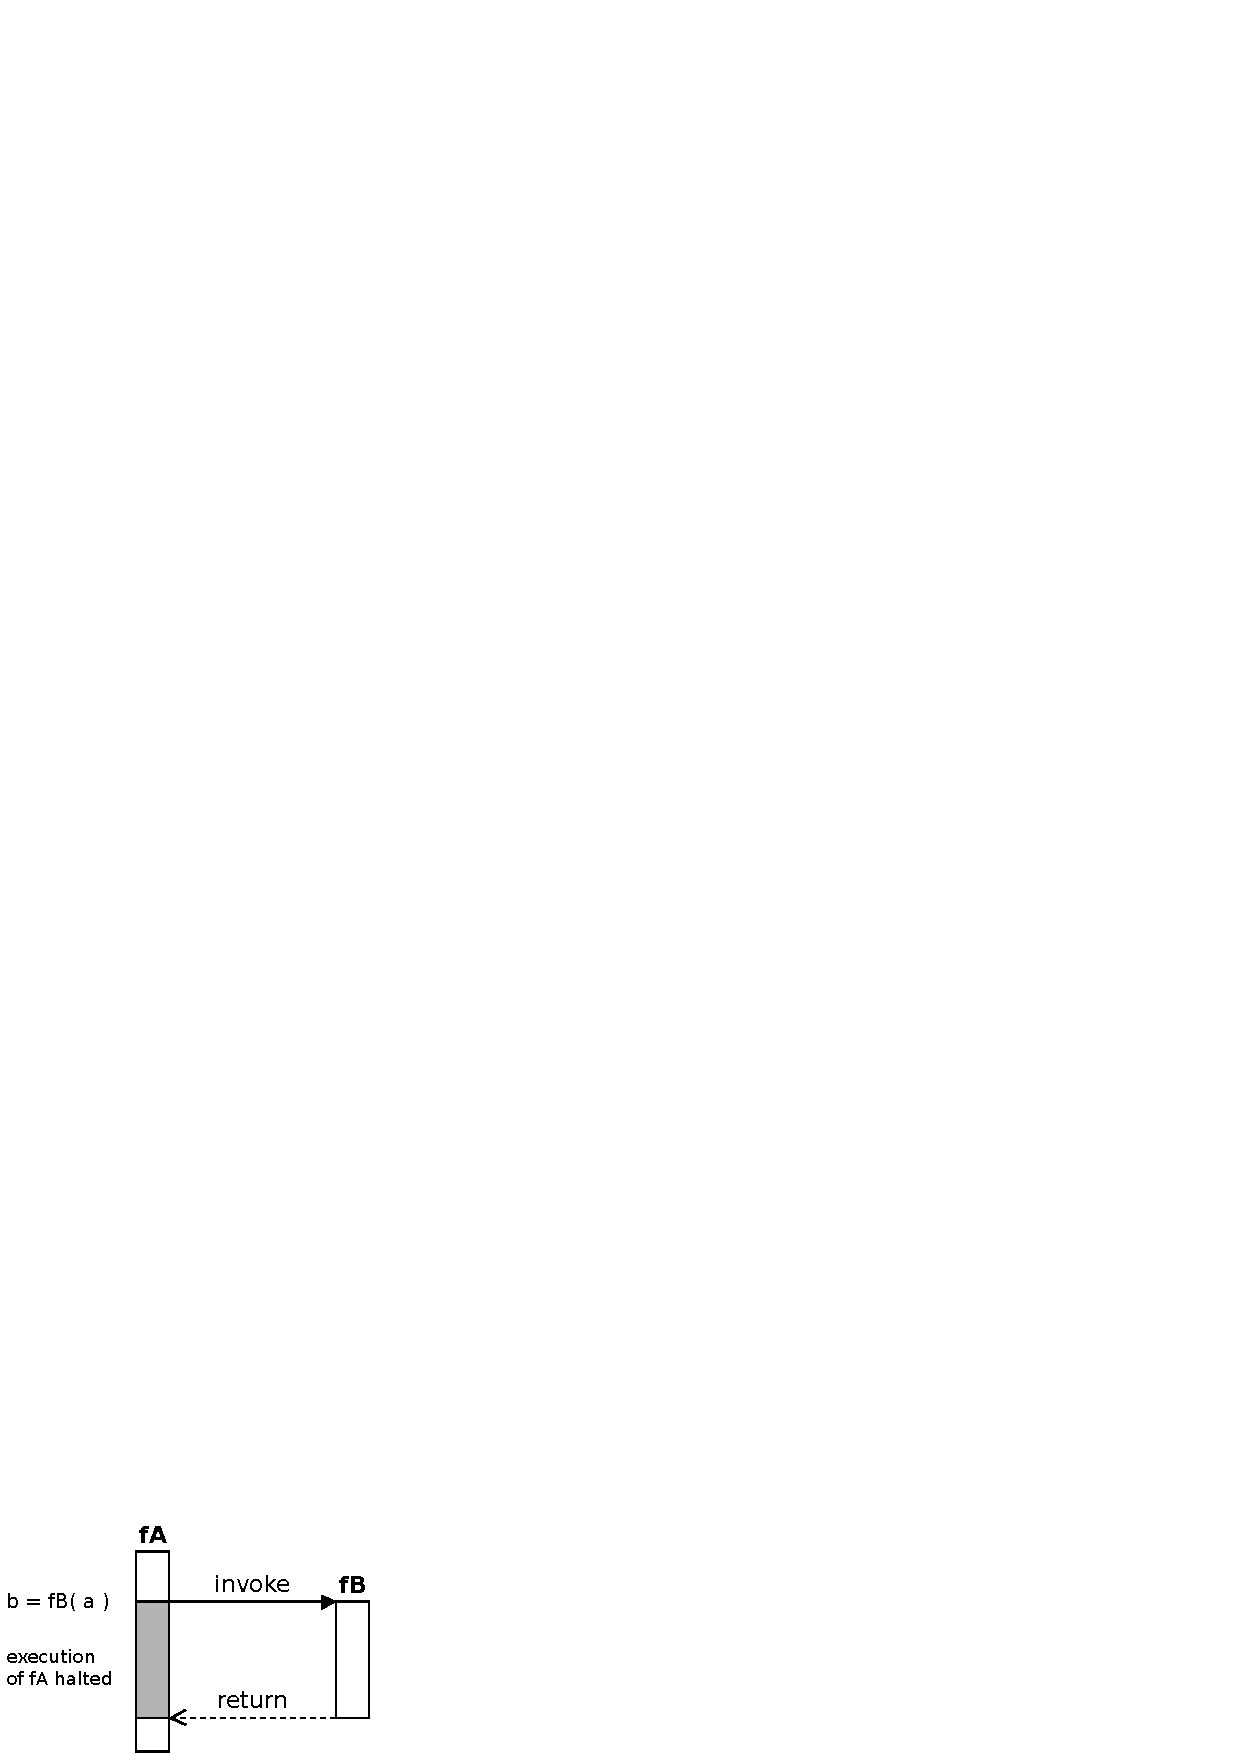
\includegraphics{figures/Closures_Synchronous}
	\caption{Synchronous Function Call}
	\label{fig:Closures_Synchronous}
\end{figure}

Asynchronous code execution, as shown in Figure~\ref{fig:Closures_Asynchronous}, allows non-blocking and thus scalable applications.
Non-blocking operations are a remedy for optimized resource allocation and open up ways to overcome previously described unnecessary resource bindings.
Processing any kind of latency-driven I/O operation asynchronously ( e.g. filesystem access and socket communication ) exploits resources that would otherwise be bound while waiting for completion.
Such operations are processed and completed whenever required resources are available.
\begin{figure}[!ht]
	\centering
  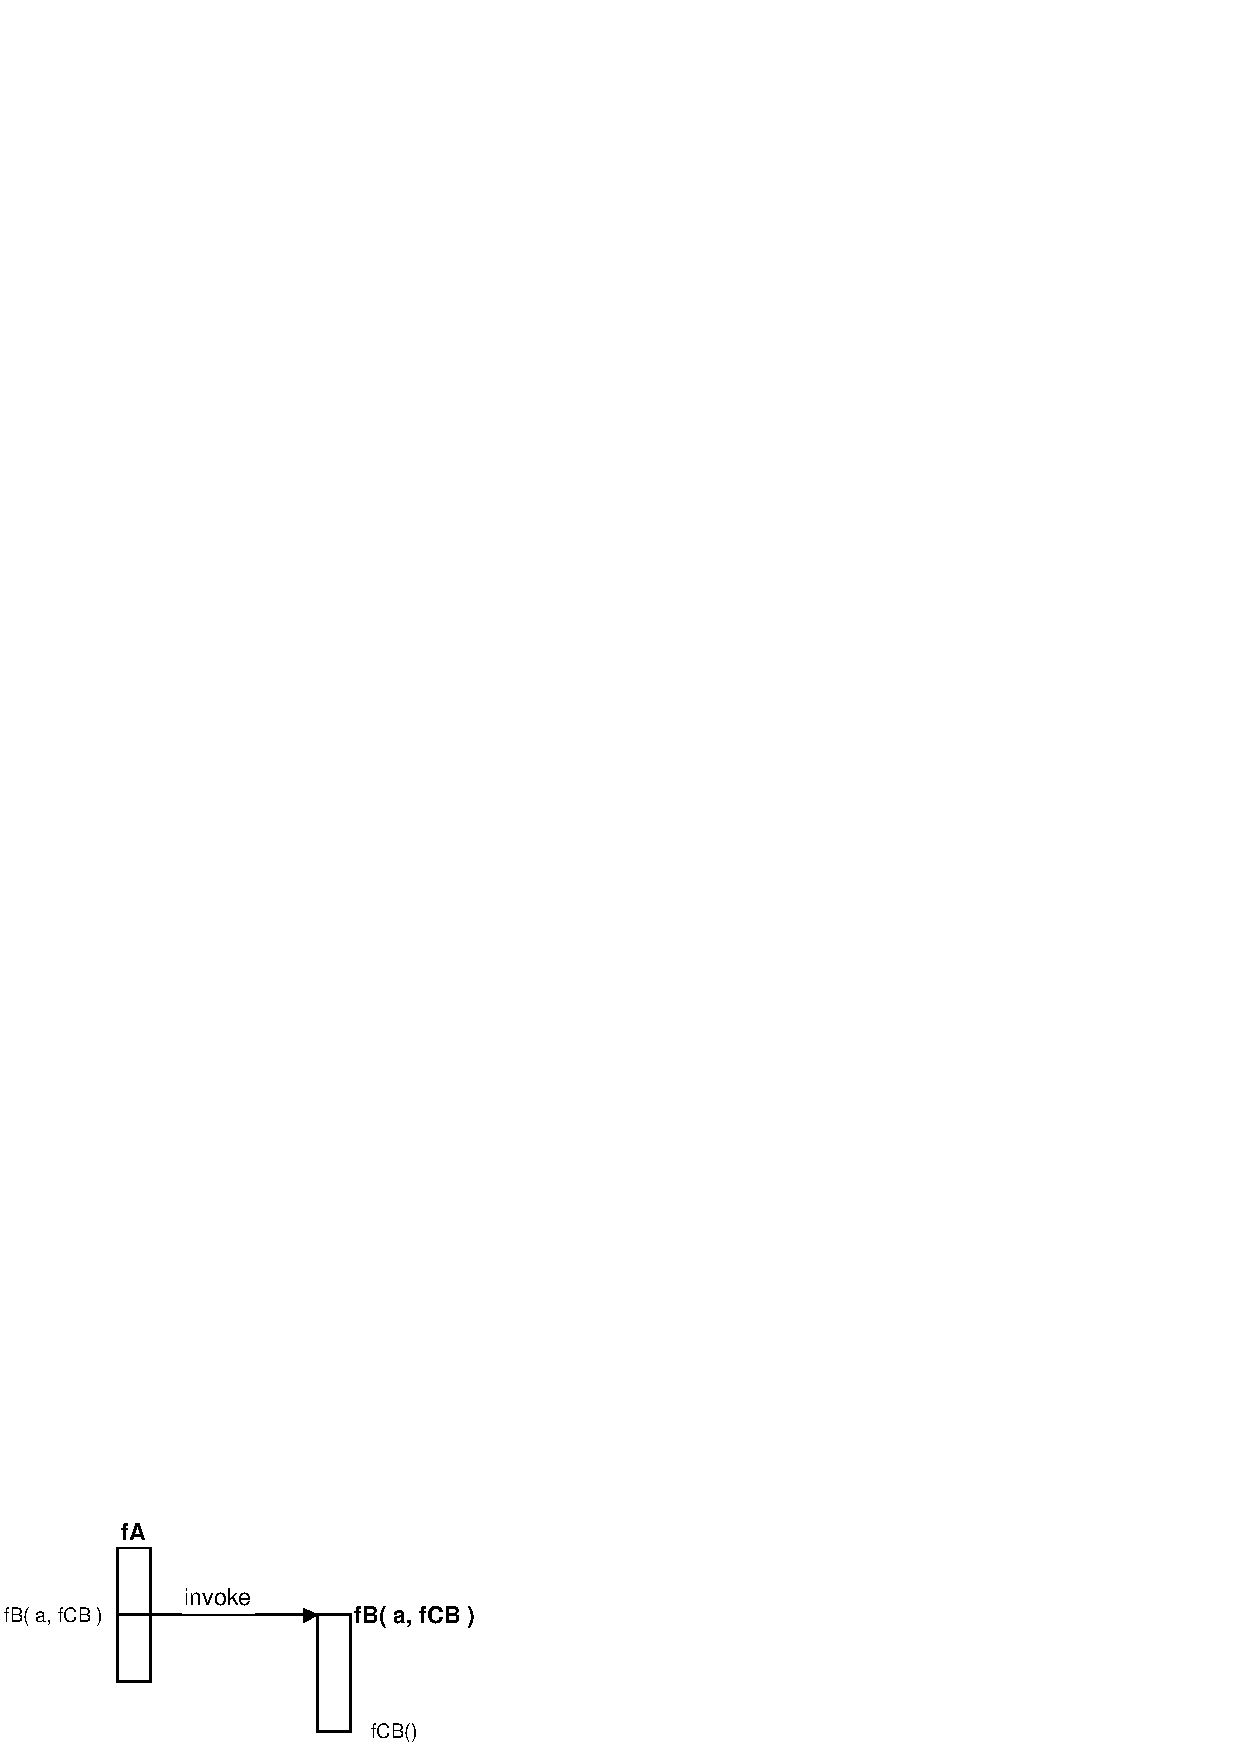
\includegraphics{figures/Closures_Asynchronous}
	\caption{Asynchronous Function Call}
	\label{fig:Closures_Asynchronous}
\end{figure}

Often other operations depend on the completion of asynchronous operations, hence their execution needs to be deferred.
This necessary code execution deferral is achieved through the use of callback functions, denoted \texttt{fCB} in Figure~\ref{fig:Closures_Asynchronous}.
Any code placed in a callback function, which is assigned to an asynchronous operation, is only executed after the respective asynchronous operation completed.
% TODO figure: Callback; Result ensurance (ergebnissichherung) wird direkt mit funktion mitgeschickt
This allows stacking of functions and operations upon each other which automatically results in a flexible and event-driven application.

So far we did not regard the context for such asynchronous functions.
If a function has access to the enclosing context where it was invoked in, it is called a closure.
Closures play an important role in \textrm{ECMAScript}\cite{EcmaScript}, which is the base for widely-spread script languages like JavaScript, JScript and ActionScript.
Closures in \textrm{ECMAScript} are defined such as they have access to the context of the function they were created in.
This is shown in Figure~\ref{fig:Closures_Closure-1} where \texttt{c} from \texttt{fA}'s context is accessible from within \texttt{fB}, assuming that \texttt{fB} was created in \texttt{fA} and not only invoked from there.
Closures make it necessary for the context of the outer function to survive past its execution so no references are broken.
This is labeled "extended context lifetime" in Figure~\ref{fig:Closures_Closure-1}.
Using asynchronous closures it becomes evident, that the context in the invoking function can change while the closure is still computing and eventually referencing the outer context, thus causing race conditions.
This will be most obvious in a loop that immediately invokes \texttt{fB} several times, as shown in Figure~\ref{fig:Closures_Closure-2}.
In such a setup \texttt{c} will have different values in the same part of different invocations of \texttt{fB}.
\begin{figure}[!ht]
	\centering
  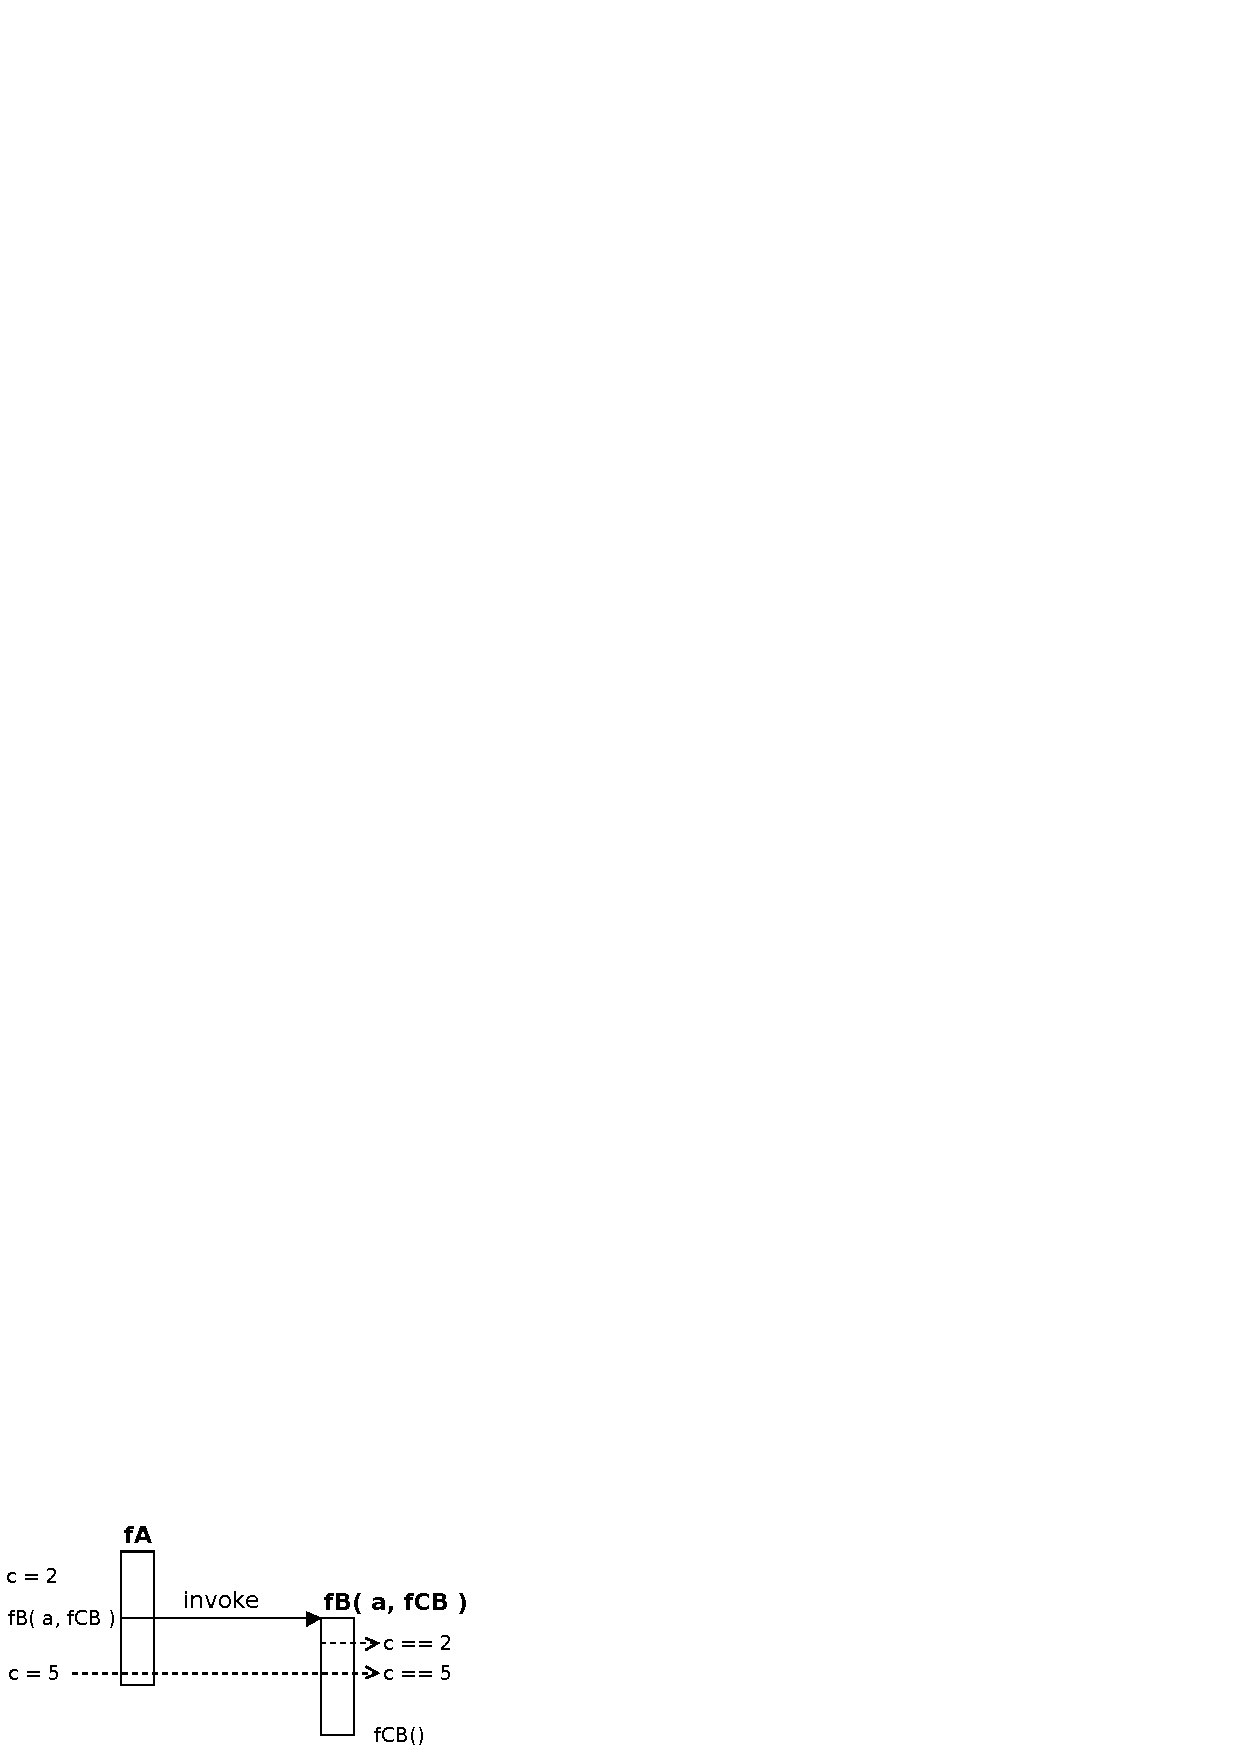
\includegraphics{figures/Closures_Closure-1}
	\caption{Closure Scope and referenced context}
	\label{fig:Closures_Closure-1}
\end{figure}
\begin{figure}[!ht]
	\centering
  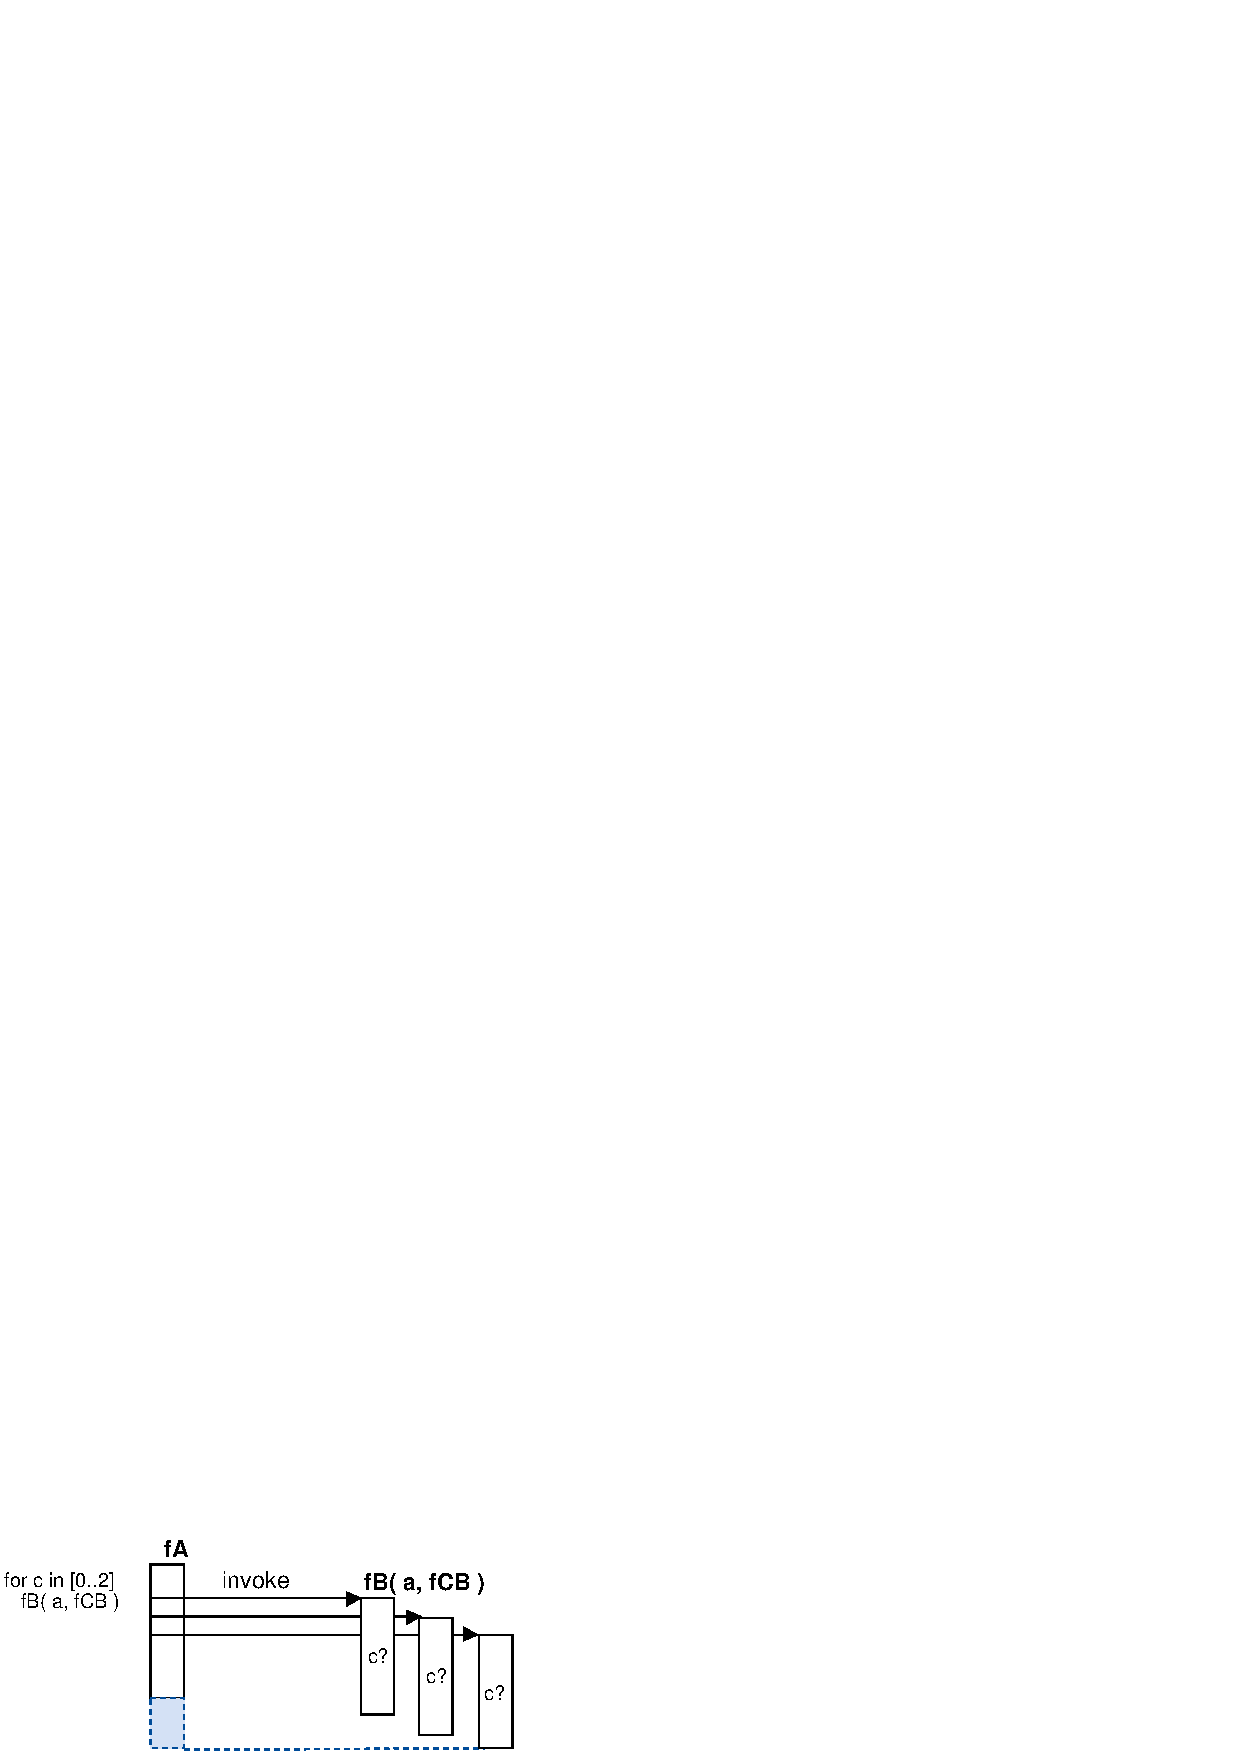
\includegraphics{figures/Closures_Closure-2}
	\caption{Closure context changes in a loop}
	\label{fig:Closures_Closure-2}
\end{figure}


Those event-driven context overwrites can be taken care of by shielding the closure from context changes, as shown in Figure~\ref{fig:Closures_Closure-3}.
To shield the closure form context changes, closure \texttt{fB} needs to create another closure \texttt{fC} and return it to \texttt{fA}.
The argument passed to \texttt{fB} is the context ( \texttt{c} in Figure~\ref{fig:Closures_Closure-3} ) that might change but requires to be persistent for one invocation.
\texttt{fC} has now \texttt{c} as a fixed context, which ca not be overwritten anymore.
Now the only thing left is \texttt{fC} needs to be invoked and it will retain the original context.
This implementation is necessary when the closure acts as a callback function for asynchronous operations, to preserve the original context in case it is required within the callback function.
\begin{figure}[!ht]
	\centering
  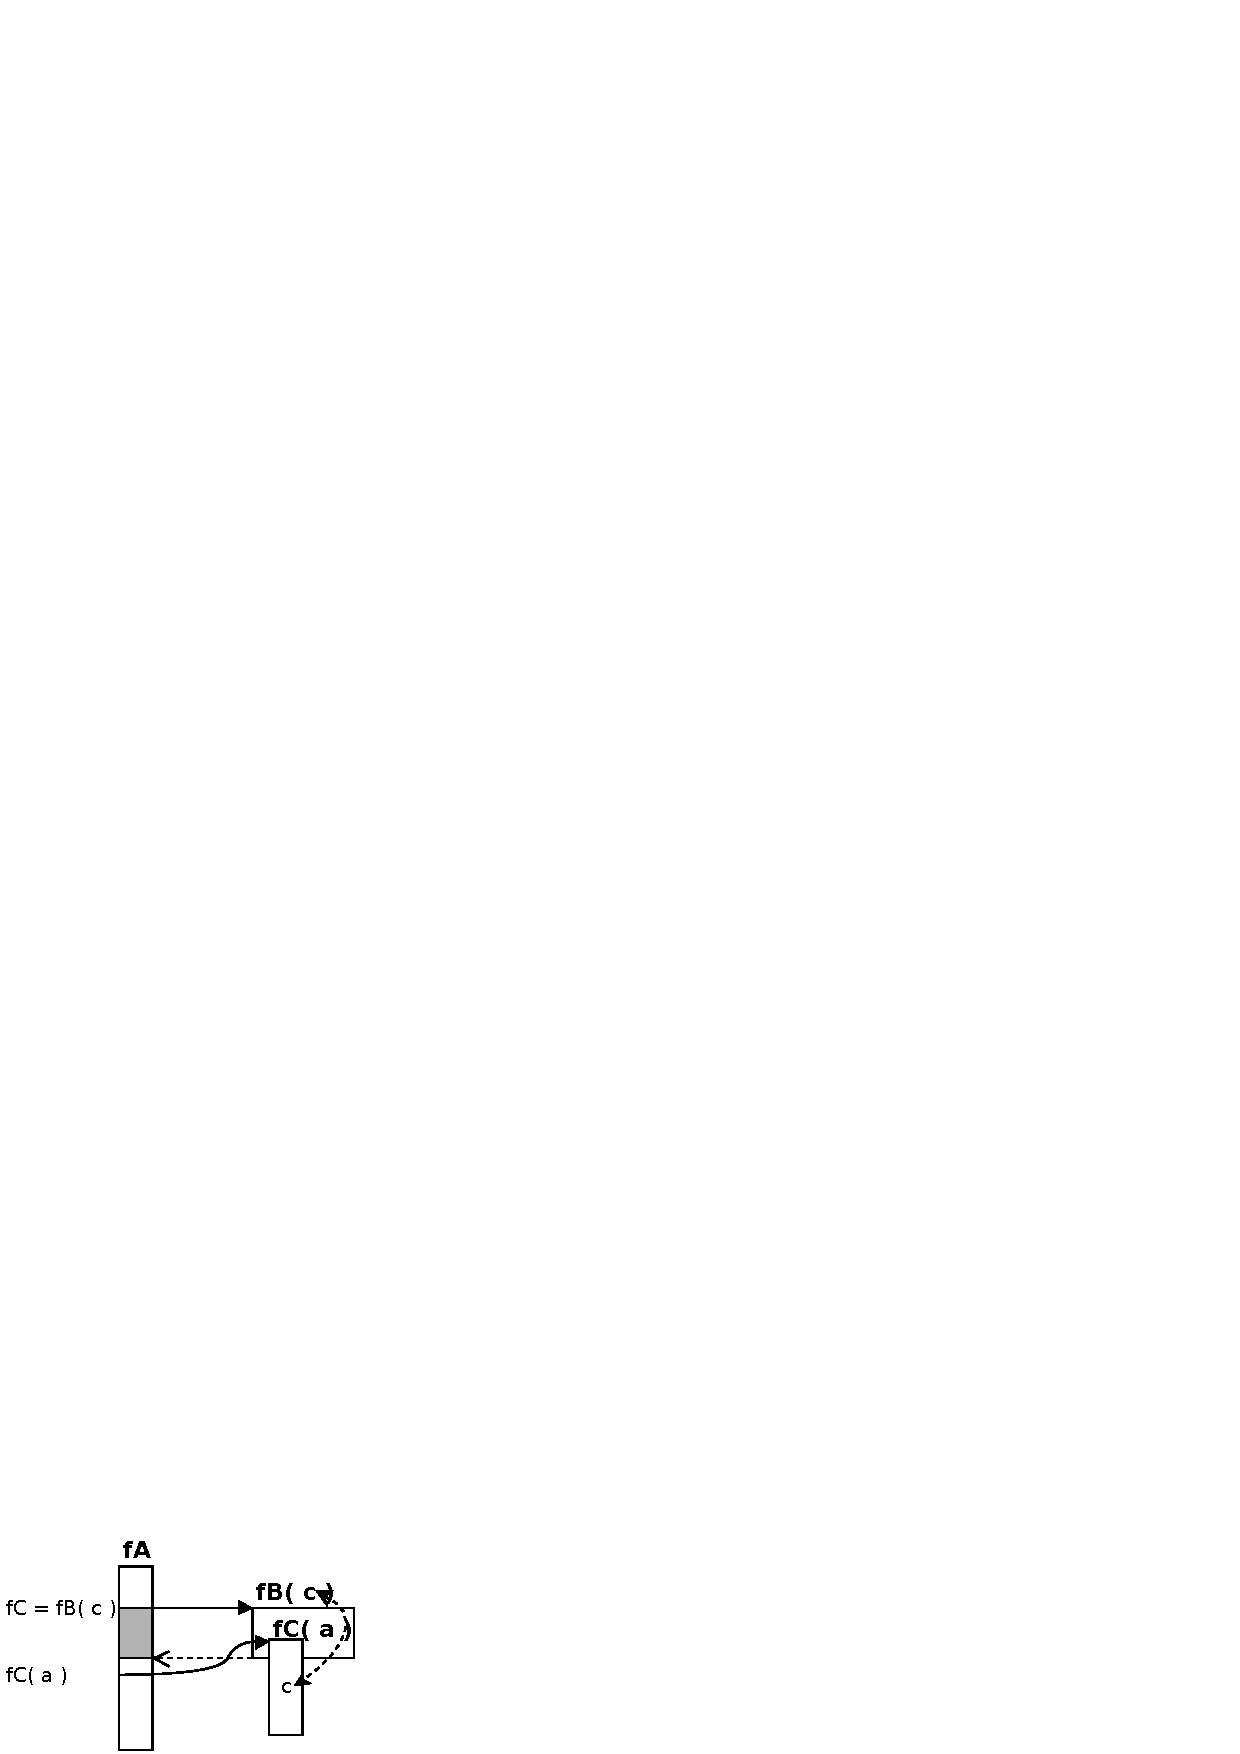
\includegraphics{figures/Closures_Closure-3}
	\caption{Closure Context Shielding}
	\label{fig:Closures_Closure-3}
\end{figure}

% TODO Figures need fA to be right aligned

An example of how closure contexts can be shielded is shown in the Listing \ref{lst_closure}.
\begin{lstlisting}[float=h,label=lst_closure,language=JavaScript,caption=JavaScript Closure Context Shielding]
var fB = function( c ) { // Declare a function...
	var fC =  function( a ) { // ( <-- function to return )
		console.log( c );
	};
	return fC;
};
for( var c = 0; c < 100; c++ ) {
	// ... before you assign it to an event happening in the future:
	var fC = fB( c );
	setTimeout( fC, 3000); // will be executed after the loop ended
}
\end{lstlisting}



	
\chapter{Conclusions \& Future Work}
% what reached, how to go on?

% Why is our system required, compare to servlets in terms of dynamic loading? user specific
% in the future what about somebody discovering our system as worthy to push events to? -> needs detection of new events

% \section{Use Cases}
% NOTES / TODOs:
%
% Temperature warning, using import.io
% Tutorial example: as seen by user, as seen by the developer
%http://khanlou.com/2014/03/model-view-whatever/
% Transactions in businesses, find use case. how would we lose events?


% We are taking a step further and allow not only the chaining up of several remote ECA engines, but also the invocation of actions on any arbitrary Web accessible service.


% TODO Use Case ( examples concrete )
% TODO Future Work

% NOTES / TODOs:
%
% CEP
We have seen that the ECA approach is already a powerful one to make the Web reactive.
A future improvement of this could be to adopt Complex Event Processing (CEP).
This would mean that several events could be stored in a rule and be evaluated in terms of time constraints.
Through this more complex events can be created as a result of several atomic events which would lead into semantically more complex events.
A change in paradigm will result in an approach where events are not just processed when they are entering the system and evaluated against rules, but these events would need to be stored for quite a long time.
Also the rules will not all be checked for each event but they are subject to a scheduler.
It can be decided when and how often a rule is evaluated and all events will be checked at these point in times, whether they are candidates for firing the rule.
A relational database will be needed in order to search through the timestamps

% Transactions for business. find use case.and explain how we would loose events.
% TODO pathologische beispiele
% Endless loops -> child_process to be killed when not responding. what about async callbacks?

% Scheduler


% CEP
%CEP has received a lot of attention

% \cite{robins2010complex}
% This paper examines the foundations and state of the research in
% Complex Event Processing (CEP), a layer built on top of Event
% Driven Architecture (EDA).
%% CEP bases on event-driven architecture
% From this viewpoint, CEP can be regarded as a service that receives and matches lower-level events and generates higher-level events, 
% if we implement event templating with properties such as described in 

Definition of events\cite{Adaikkalavan2007}

% RDFTL: The condition part is a query which de-
% termines if the information system is in a particular state, in which case the rule fires.

% TODO Condition evaluation on other resources? i.e. make a request to a remote site and evaluate it? -> also achievable through composite events

% \index{CEP}
% \index{Composite Events}
% We will then continue by introducing the Event-Conditon-Action (ECA) paradigm and its umbrella term complex event processing (CEP) as approach to impose reactivity.

% CEP or Composite event detection~\cite{Gehani92compositeevent}~\cite{2004_1265833}~\cite{2006Muehl}~\cite{demers2007cayuga}~\cite{akdere2008plan}~\cite{anicic2010arlfcepar}

% automatic detection of new events within the system and information about them to the user
% the system needs to learn about events

% If we go to the semantic web we could incorporate RDF queries in order to allow smart event distinction

% web resurce (URI) can be data but also well defined service through REST. incorporating web resources into model 

 % conditions as web queries can be solved through event composition
% show rule engines, alsoo CEP, describe event composition through templates and why we don't do it


% Bibliography
	\addcontentsline{toc}{chapter}{Bibliography}
	\bibliography{thesisbib}
	\bibliographystyle{thesisbst}

% Lists
	\listoffigures
	% FIXME CHECK WHETHER TABLES OR LISTINGS ARE IN THE DOCUMENT
	\listoftables
	% \lstlistoflistings

% Index
	\addcontentsline{toc}{chapter}{Index}
	\printindex

	% Turn off listing of tables and figures since from here on they will be in the appendix
	\captionsetup[figure]{list=no}
	\captionsetup[table]{list=no}

% Appendix
	\begin{appendices}
	\addtocontents{toc}{\setcounter{tocdepth}{-1}}
	
\chapter{Use Case Code}


\section{Application to Ping IPs and push Result to Remote Server}

\begin{lstlisting}[nolol,language=CoffeeScript,label={lst:eventproducer}]
fs = require 'fs'
ping = require 'net-ping'
needle = require 'needle'
    
remoteUrl = "http://ec2-54-196-2-15.compute-1.amazonaws.com"
fPushEvent = ( evt ) ->
  needle.post remoteUrl + '/measurements', JSON.stringify( evt )

try
  histData = fs.readFileSync 'histoappend.json', 'utf8'
catch err
  console.error "Error reading historical data file"
  process.exit()

session = ping.createSession retries: 2
oSum = {}
if histData
  arrPings = histData.split "\n"
  try
    for strObj, i in arrPings
      if strObj isnt ''
        oTmp = JSON.parse strObj  
        oSum[ oTmp.timestamp ] = 
          sum: oTmp.sum
    if oTmp
      fPushEvent
        currentlyon: oSum[ oTmp.timestamp ].sum
        pingtimes: oSum   

  catch err
    console.log 'Error parsing histo data'
    console.log err

i = -1
ips = []
pingTime = (new Date()).toISOString()
fPollHosts = () ->
  i++
  session.pingHost "131.152.85.#{ i }", ( err, target, sent, rcvd ) ->
    if not err
      ips.push target
      
  if i is 255
    i = -1
    console.log "#{ (new Date()).toISOString() } | All ping requests returned (#{ips.length} answered), pushing event into the system and starting again at 0"
    
    oSum[ pingTime ] = sum: ips.length
    fPushEvent JSON.stringify
      currentlyon: ips.length
      pingtimes: oSum

    oPing = 
      timestamp: pingTime
      ips: ips
      sum: ips.length

    fs.appendFile 'histoappend.json', JSON.stringify( oPing ) + "\n", 'utf8'
    pingTime = (new Date()).toISOString()
    ips = []


  setTimeout fPollHosts, 7000


fPollHosts()


\end{lstlisting}

	
\chapter{Rules}
\section{Binder Annotations}
\subsection{Binder Annotations}


	
\chapter{Benchmarking}
\section{Java}

\begin{lstlisting}[nolol,label=lst_bm_java,language=Java,caption=Closure Benchmarking: Java Code]
/*
 * BenchmarkingDeferred.java
 */
import java.util.concurrent.ScheduledExecutorService;
import java.util.concurrent.Executors;
import java.util.concurrent.TimeUnit;
import java.util.HashMap;

public class BenchmarkingDeferred {

  private static Runtime runtime = Runtime.getRuntime();
  private static final ScheduledExecutorService worker = 
    Executors.newSingleThreadScheduledExecutor();

  private static void deferFunctionCall( int numScopeVars, int delay, String scopeId ) {
    HashMap<String, String> mapVars = new HashMap<String, String>();
    for( int i = 0; i < numScopeVars; i++ ) {
      mapVars.put( "id" + i, "12345678" ); // 8 bytes per stored scope variable
    }
    Object context = new TimeoutContext( "TimeoutFunction" );
    Runnable task = new RunnableCallbackFunction( mapVars, context );
    worker.schedule( task, delay, TimeUnit.SECONDS );
  }

  public static void main( String[] args ) {
    long startTime, stopTime;
    int numVars = 10, firstArg = 0;
    firstArg = Integer.parseInt( args[0] );
    numVars = Integer.parseInt( args[1] );
    int j = 0, numFuncs = 1 << firstArg;

    startTime = System.nanoTime();
    while( j++ < numFuncs) {
      deferFunctionCall( numVars, numFuncs * 10, numFuncs + "(" + j + ")" );
    }
    stopTime = System.nanoTime();

    // [...] benchmark system out

    worker.shutdownNow();
  }
}

/*
 * RunnableCallbackFunction.java
 */
import java.util.HashMap;

/*
 * The Callback function instance.
 */
public class RunnableCallbackFunction implements Runnable {
  
  // The hashhmap is used to store variables and their value as the scope
  private HashMap<String, String> mapScope;
  private Object context;

  public RunnableCallbackFunction( HashMap<String, String> scope, Object context ) {
    this.mapScope = scope;
    this.context = context;
  }

  // If this is executing, we did not wait long enough and the
  // benchmark time is compromised
  public void run() {
    System.out.println( mapScope.toString() );
  }

}

/*
 * TimeoutContext.java
 */
public class TimeoutContext {
  private long idleTimeout = 1;
  private long idlePrev;
  private long idleNext;
  private long idleStart = 140000505;
  private String onTimeout = null;
  private boolean repeat = false;

  public TimeoutContext( String cb ) {
    this.onTimeout = cb;
  }
}

\end{lstlisting}

\section{JavaScript}
\begin{lstlisting}[nolol,float=h,label=lst_bm_js,language=JavaScript,caption=Closure Benchmarking: JavaScript Code]
/*
The function deferral measurements in node.js
*/

var deferredFunction = function ( numScopeVars, delay, scopeId ) {
  var scope = {};
  for ( var i = 0; i < numScopeVars; i++ ) {
    scope[ "id" + i ] = "12345678"; // 8 bytes per stored scope variable
  }
  setTimeout( function () {
    // If this is executed we did not wait long enough
    console.log( JSON.stringify( scope, null, '  ' ) );
  }, delay );
}

var numOfFunctions,
    numOfScopeVars = process.argv[ 3 ];

numOfFunctions = Math.pow( 2,  process.argv[ 2 ] );

var time = process.hrtime();
for (var i = 0; i < numOfFunctions; i++) {
  deferredFunction( numOfScopeVars, 1000 * numOfFunctions, numOfFunctions + "(" + i + ")" );
};
var diff = process.hrtime( time );

var mem = process.memoryUsage();
// [...] benchmark system out
process.exit( 0 );

\end{lstlisting}

	
	\end{appendices}

	\addtocontents{toc}{\setcounter{tocdepth}{1}}

\backmatter
	
\pagestyle{empty}
\begin{figure}[!ht]
	\begin{adjustwidth}{-\oddsidemargin-1in}{-\rightmargin}
		\centering
		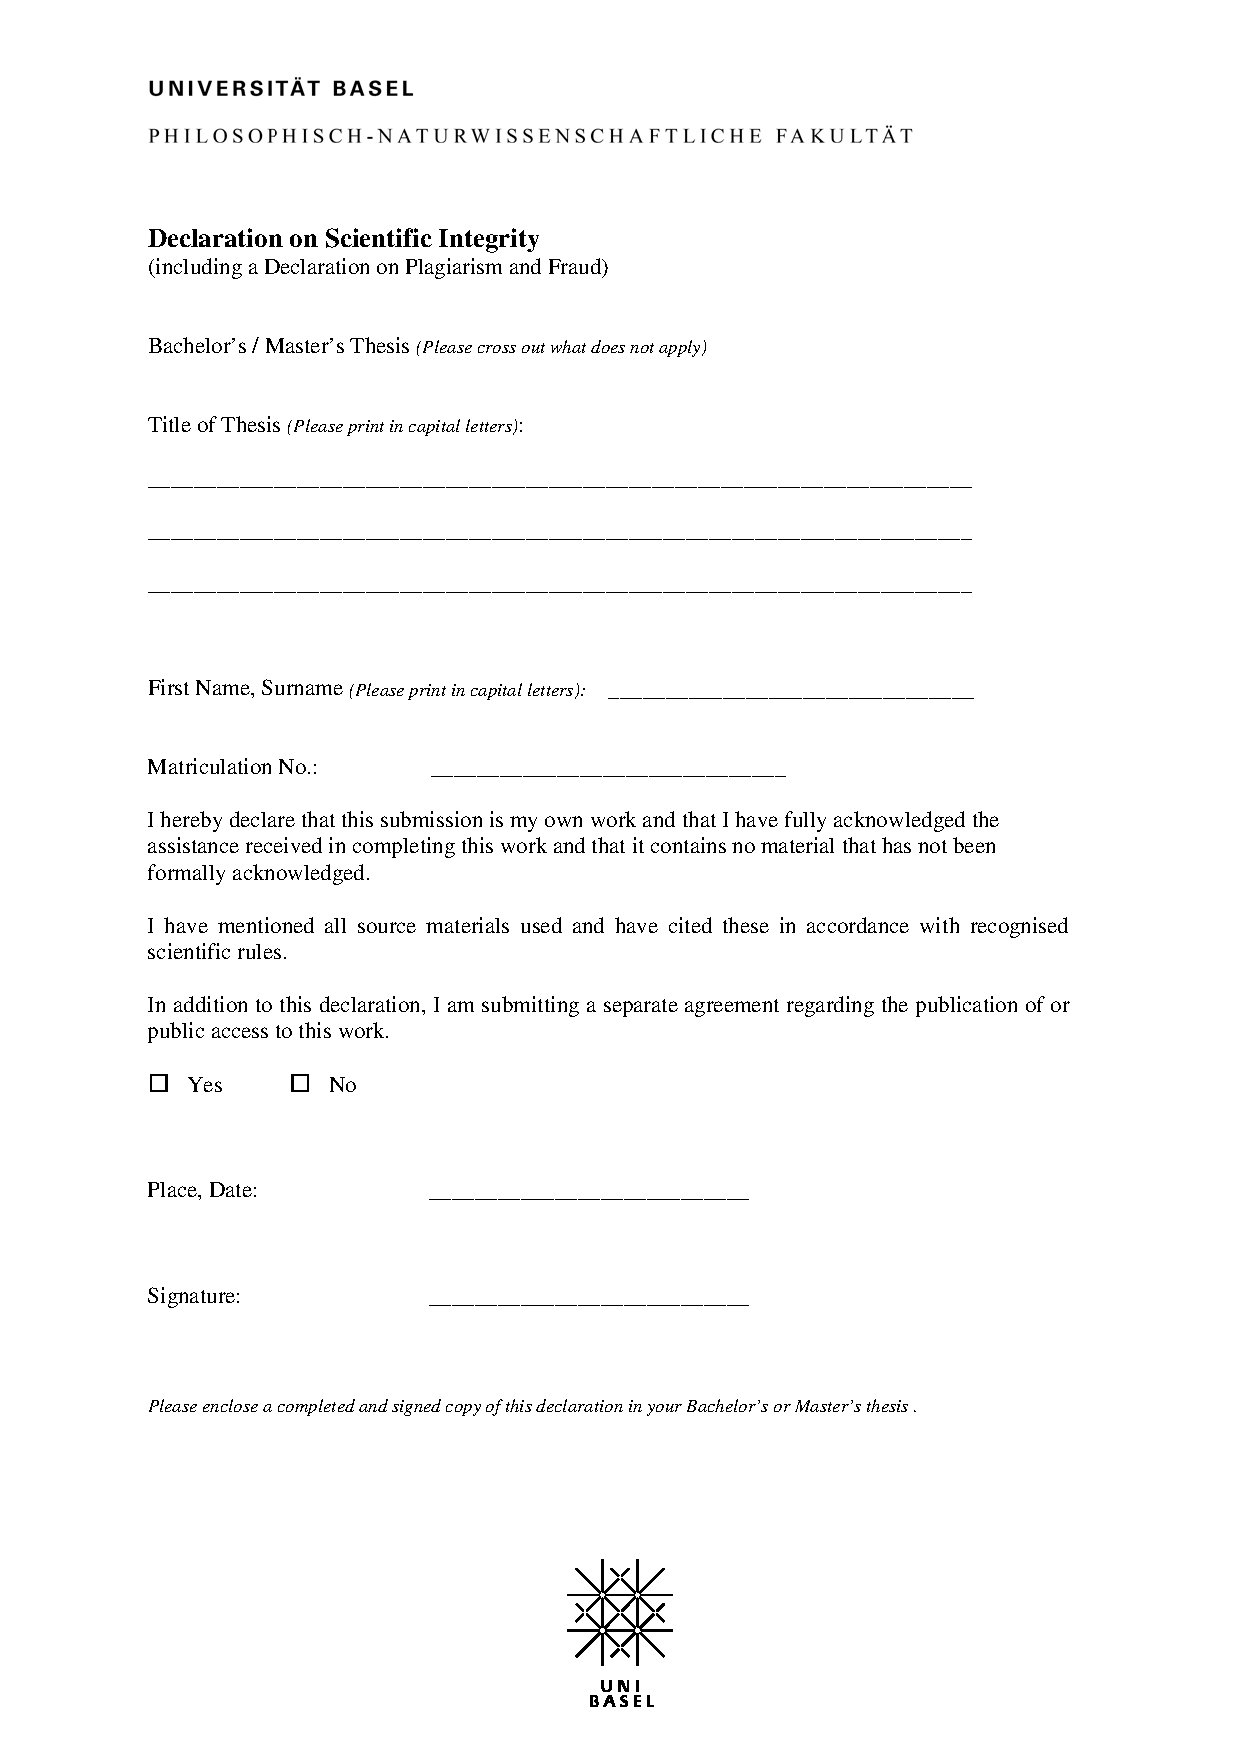
\includegraphics[width=\paperwidth]{figures/scientificintegrity}
	\end{adjustwidth}
\end{figure}
% 	\addtocontents{toc}{\setcounter{tocdepth}{1}}

\end{document}
